% ------------------------------------------------------------------------------
% CAPÍTULO 7 -------------------------------------------------------------------
% ------------------------------------------------------------------------------
\chapter{Integración y validación de la placa de expansión Flow Deck}
En este capítulo se presenta una explicación detallada del procedimiento realizado para lograr la integración exitosa de la placa de expansión Flow Deck en el dron Crazyflie 2.1. Para realizar esta tarea, se utilizó un ordenador con sistema operativo Windows 11 y \textit{software} de código abierto proporcionado por el grupo Bitcraze. También, se describen los experimentos de vuelo reaizados con y sin la placa de expansión Flow Deck y se proporcionan observaciones importantes, relacionadas con el entorno de experimentación, para que la placa funcione correctamente.

\section{Validación de funcionamiento de Crazyflie}
Previo a la instalación de la placa de expansión, fue necesario realizar una verificación del ensamble y ajustes de configuración con el fin de garantizar el funcionamiento adecuado del dron Crazyflie 2.1 para los fines del proyecto.

\subsection{Ensamble de Crazyflie}
Respecto al ensamble del dron, se consultó el tutorial de armado y pruebas de vuelo disponible en la página oficial de Bitcraze \cite{Crazyflie_tutorial_ensamble}. Se examinó que cada parte del dron estuviera correctamente instalada según la información en la página. El resultado obtenido se observa en la Figura \ref{fig:Crazyflie_ensamble} donde se muestra al dron correctamente ensamblado. 

\begin{figure}[htbp]
	\centering
	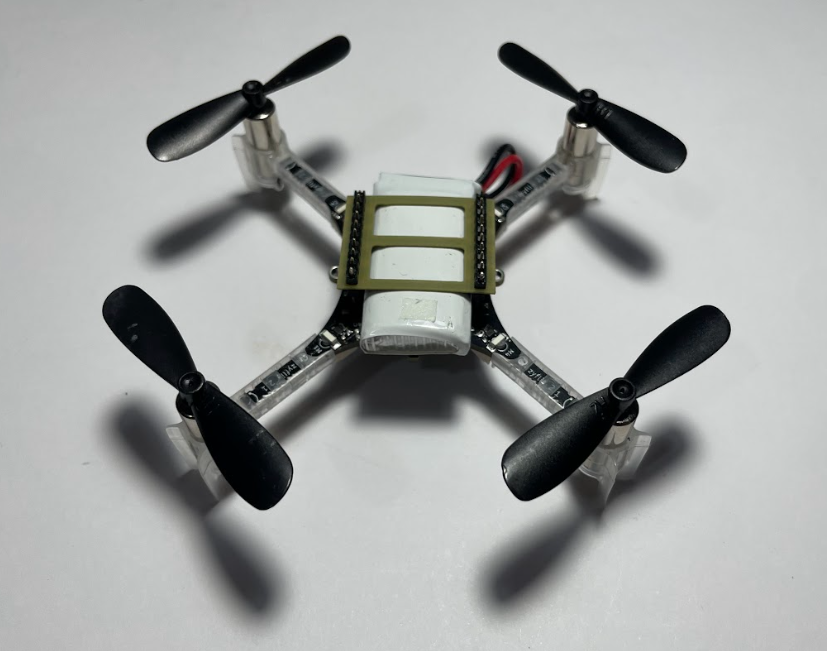
\includegraphics[width=0.4\textwidth]{Crazyflie_ensamblado}
	\caption{Ensamble correcto de dron Crazyflie 2.1.}
	\label{fig:Crazyflie_ensamble}
\end{figure}

Luego de examinar y validar el ensamble, se ejecutó la secuencia de autoprueba presionando el botón de encendido. Esta secuencia preparó al dron para volar, verificando que el \textit{hardware} se encontrara en buen estado y calibró los sensores con valores base. Para ejecutar la prueba, se colocó al dron en una superifice nivelada y se mantuvo absolutamente quieto.

La ejecución de la autoprueba indicó que el estado del dron se encontraba a la perfección y listo para volar. Esto se determinó con la siguiente lista de resultados que se interpretan con la modalidad de encendido de los LED presentes en el dron:
\begin{itemize}
	\item \textbf{Encendido y listo para volar:} LED azules permanecen encendidos y el LED delantero derecho parpadea en rojo dos veces por segundo.
	\item \textbf{Encendido pero con sensores descalibrados:} LED acules permanecen encendidos y el LED delantero derecho parapadea en rojo cada dos segundos.
	\item \textbf{Crazyradio conectada:} LED delantero izquierdo parpadea en rojo y/o verde.
	\item \textbf{Batería baja:} LED delantero derecho permanece completamente encendido en rojo.
	\item \textbf{Carga:} LED azul izquierdo parpadea mientras que el LED azul derecho está encendido.
	\item \textbf{Modo cargador de arranque:} LED azules parpadean una vez por segundo.
	\item \textbf{Error de autoprueba:} LED delantero derecho parpadea repetidamente en rojo con una pausa larga entre parpadeos.
\end{itemize}

\begin{figure}[htbp]
	\centering
	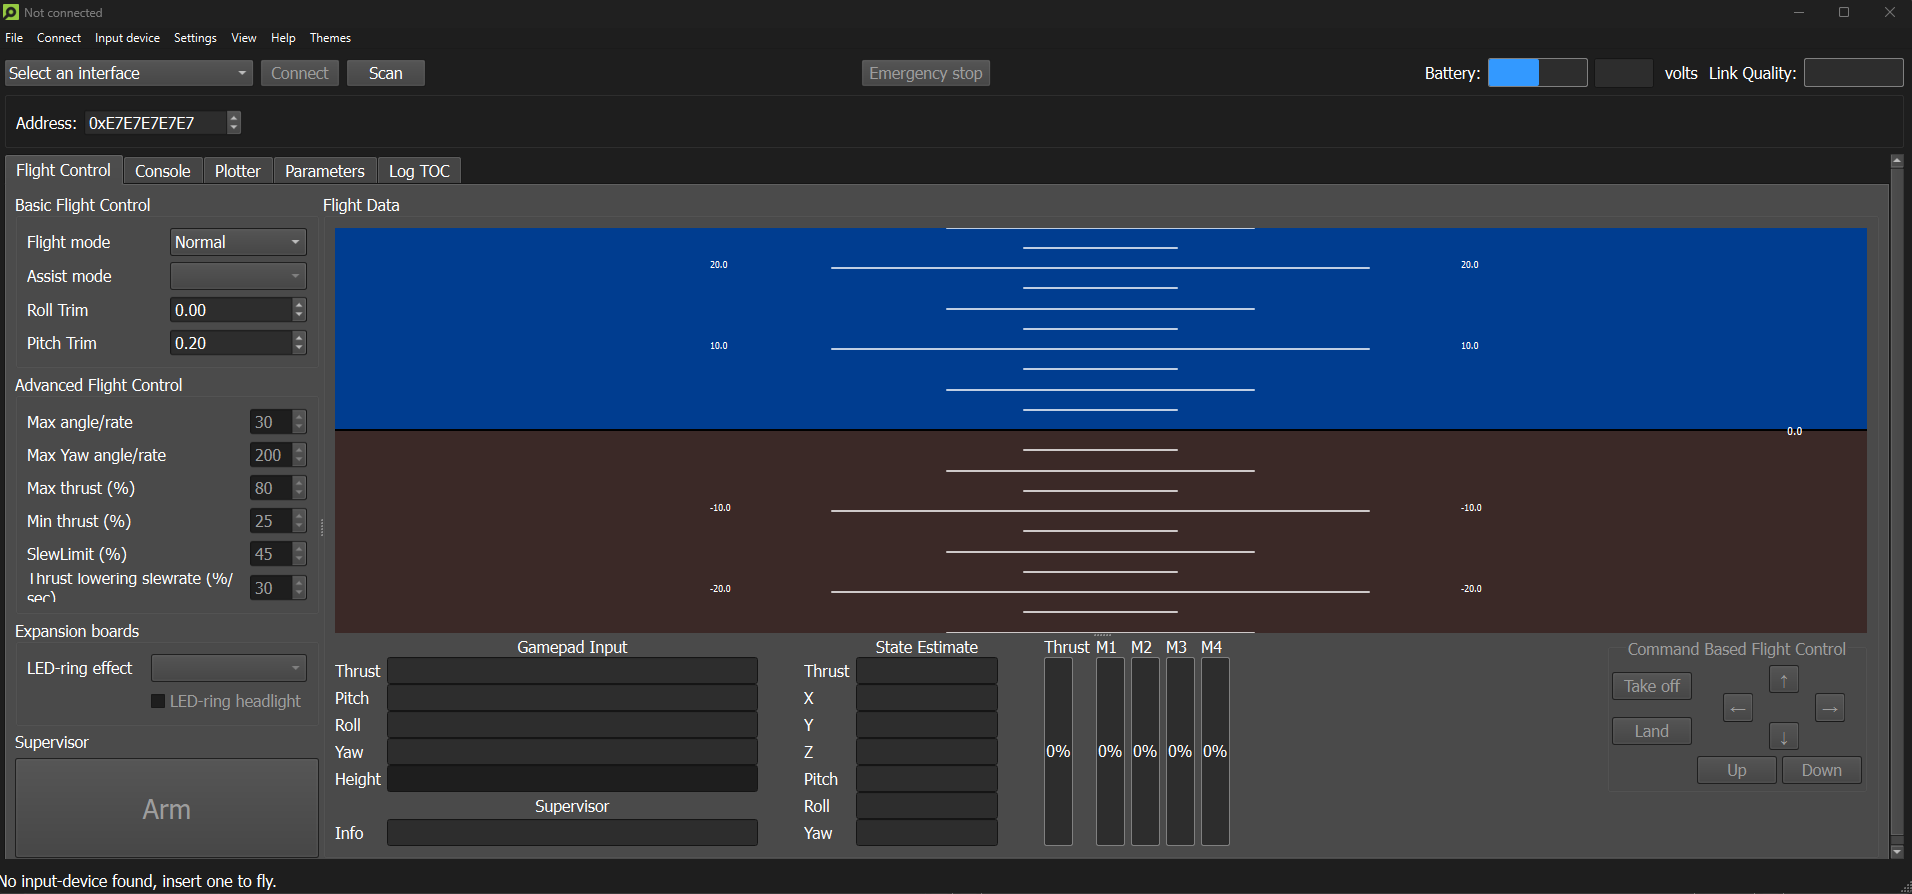
\includegraphics[width=0.85\textwidth]{Crazyclient}
	\caption{Interfaz de control de vuelo del \textit{software} Crazyclient.}
	\label{fig:Crazyclient}
\end{figure} 

\subsection{Software Crazyclient y actualización de firmware de Crazyflie}
Tras verificar que el dron iniciara correctamente, se instaló el \textit{software} de código abierto Crazyclient del grupo Bitcraze según el manual de instalación provisto en su página oficial \cite{Crazyflie_installation_Cfclient}. Se instaló la versión para Windows 10/11. Este programa dispone de diversas herramientas para el control, calibración, visualización de datos en tiempo real y configuración de parámetros del dron Crazyflie. Además, como se observa en la Figura \ref{fig:Crazyclient}, también dispone de una interfaz gráfica de usuario que facilita la interacción con el dron.

Una vez se ha instalado correctamente el programa Crazyclient, lo primero que se realizó fue la actualización de \textit{firmware} siguiendo las instrucciones en la página oficial \cite{Crazyflie_6}. Este paso es fundamental para que el dron Crazyflie sea capaz de reconocer a la placa de expansión Flow Deck. Es necesario que tenga instalada la versión más reciente disponible. para garantizar un rendimiento eficiente del \textit{hardware}.

\begin{figure}[htbp]
	\centering
	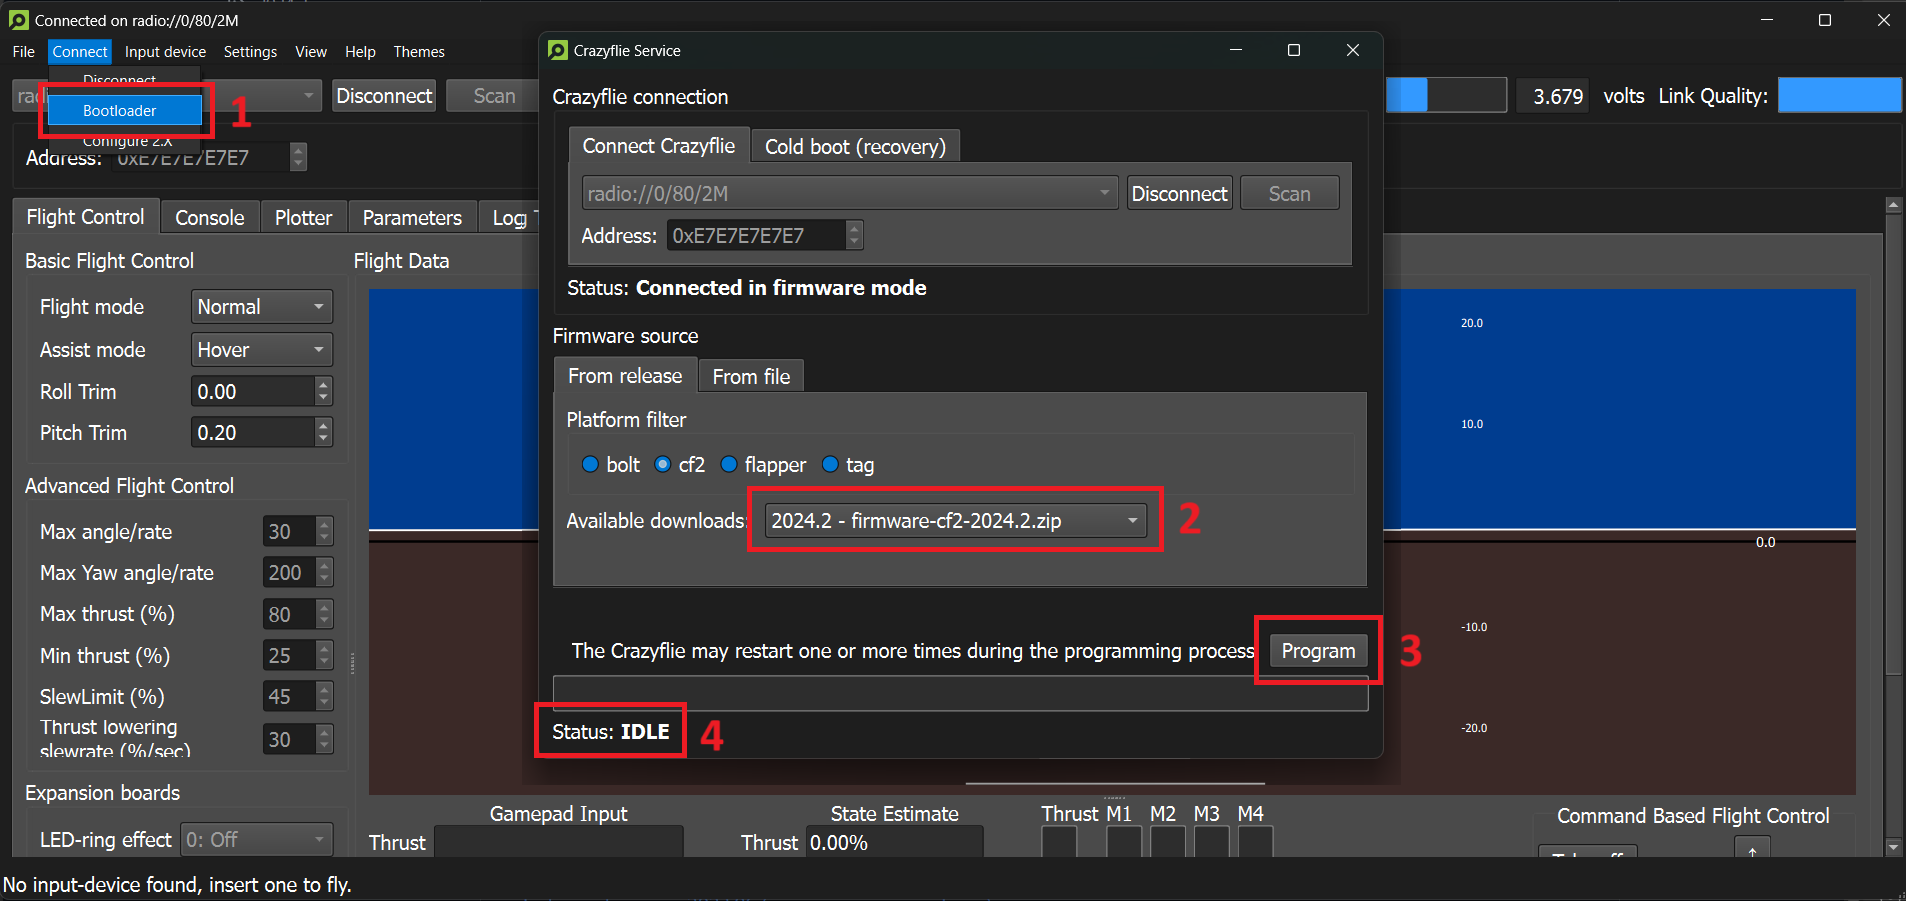
\includegraphics[width=0.85\textwidth]{Actualizacion_firmware}
	\caption{Actualización de \textit{firmware} con el programa Crazyclient.}
	\label{fig:Actualizacion_firmware}
\end{figure} 

Previo a la actualización de \textit{firmware}, fue necesario instalar los controladores USB del dispositivo Crazyradio utilizando la guía de instalación del fabricante \cite{Crazyflie_USB_driver}. Posteriormente, se empleó el Crazyradio para establecer la conexión con el Crazyflie. Una vez conectado, se siguió la serie de pasos mostrados en la Figura \ref{fig:Actualizacion_firmware}. Cabe mencionar que el último paso tan solo consiste en esperar a que termine el proceso y que el estado del dron sea IDLE. 

\subsection{Configuración de parámetros}
Como siguiente paso se habilitó la vista de parámetros del Cfclient para ajustar a los parámetros del dron con el fin de asegurar el comportamiento esperado.

\begin{itemize}
	\item \textbf{stabilizer.controller:} se colocó con un valor de 1 para utilizar el controlador PID.
	\item \textbf{stabilizer.estimator:} se colocó un valor de 2 para utilizar el estimador extendido de Kalman.
	\item \textbf{commander.enHighLevel:} se colocó un valor de 1 para permitir el envío de comandos de forma remota al dron.
\end{itemize}

\subsection{Prueba de hélices y motores}
Manteniendo la conexión del dron con el cliente, se utilizó la vista de consola para realizar una prueba de hélices y motores. Para ello, se colocó al Crazyflie sobre una superifcie plana y dura y luego se seleccionó la opción ``\textit{Propeller test}'' para realizar una prueba de vibración en motores y hélices (Figura \ref{fig:Propeller_test}). El dron accionó levemente los motores, de forma secuencial, para determinar el estado de estos y sus hélices. Para los motores que presentaron vibraciones por encima del umbral permitido se emitió un pitido y se imprimió la advertencia en consola.

\begin{figure}[htbp]
	\centering
	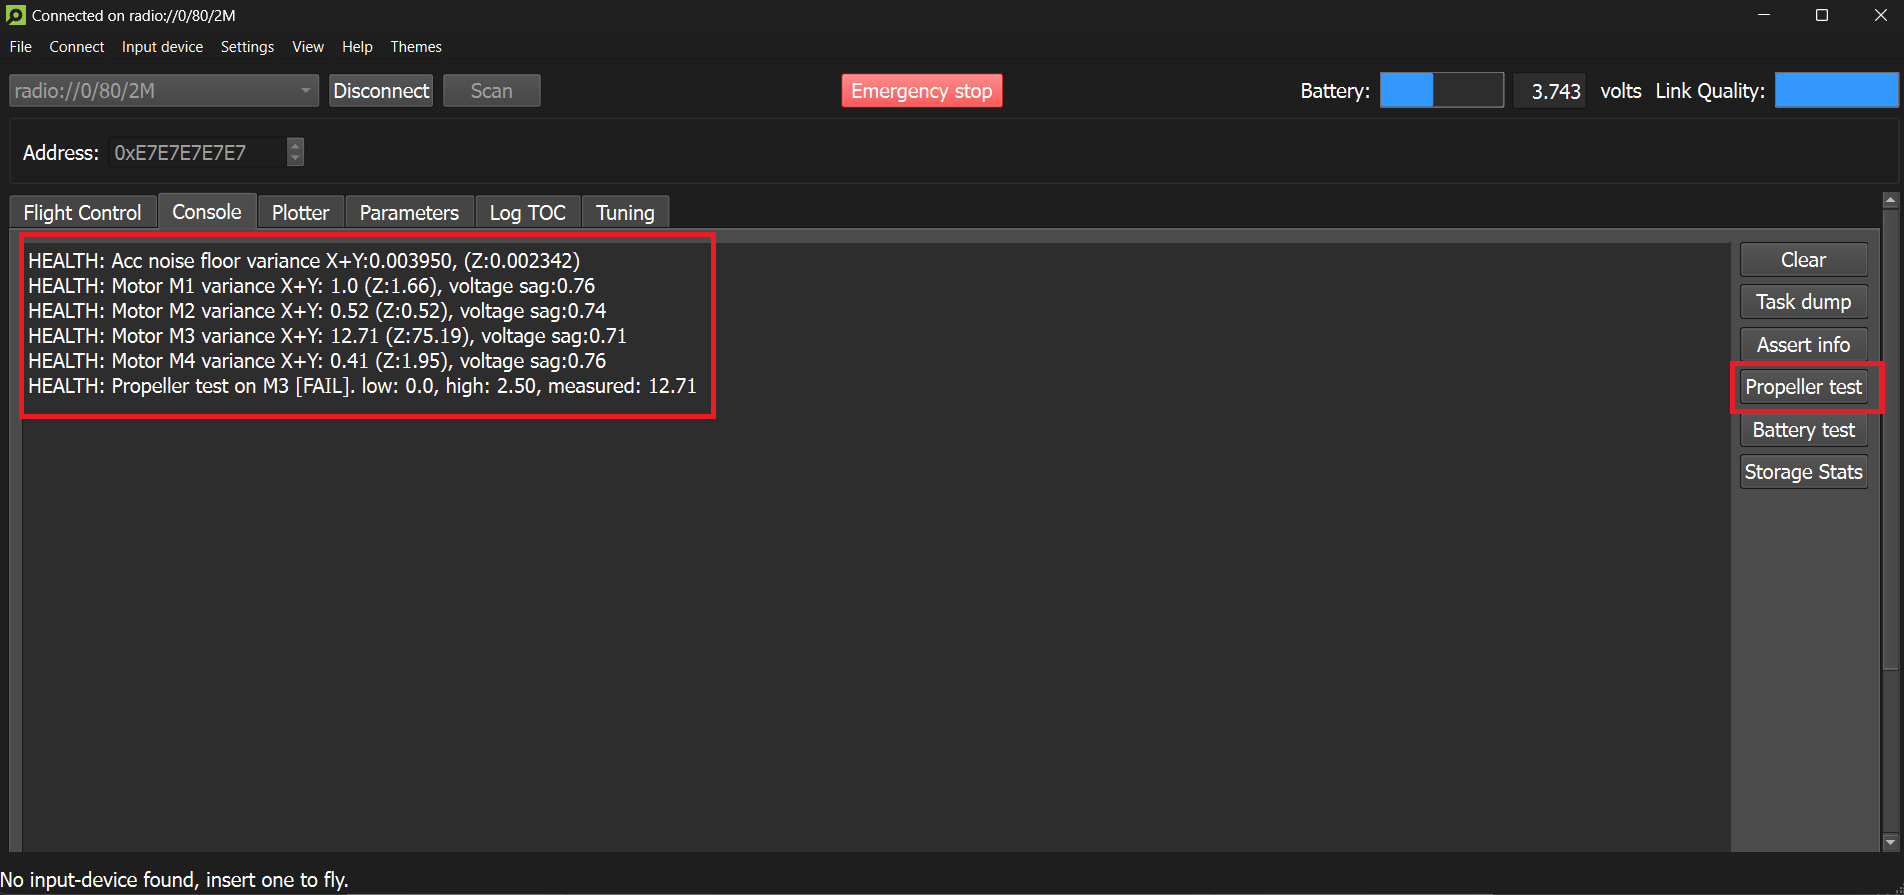
\includegraphics[width=0.85\textwidth]{Propeller_test}
	\caption{Vista de consola y prueba de vibración en hélices y motores.}
	\label{fig:Propeller_test}
\end{figure} 

Las vibraciones excesivas en los motores y hélices perjudican significativamente la calidad de vuelo del dron, por tal motivo fue necesario realizar ajustes para reducirlas o eliminarlas. Hay tres posibles soluciones al problema y deben intentarse en orden:

\begin{enumerate}
	\item \textbf{Balanceo de hélices:} La primera solución para abordar el problema es balancear las hélices, siguiendo el tutorial disponible en la página de Bitcraze \cite{Crazyflie_balancing}.
	
	\item \textbf{Reemplazo de hélices:} Si el balanceo de las hélices no resuelve el problema, se recomienda reemplazarlas con hélices nuevas de repuesto.
	
	\item \textbf{Reemplazo de motores:} Si las vibraciones persisten después de cambiar las hélices, se debe considerar el reemplazo de los motores.
\end{enumerate}

\subsection{Prueba de vuelo simple}
Luego de examinar los aspectos anteriores, se procedió a realizar una prueba de vuelo utilizando la GUI del cfclient y un mando de PS4. El objetivo del experimento fue elevar un poco el dron aplicando una cantidad considerable de Thrust para elevarlo y poder observar su comportamiento en ausencia de un sistema de posicionemiento (lazo abierto). 

El desepgue del dron fue exitoso sin embargo, como se esperaba, no logró mantener su posición durante la elevación presentando una cantidad considerable de drift y descompensación de vuelo.

\section{Instalación de la placa de expansión Flow Deck}
Habiendo verificado el funcionamiento propio del dron Crazyflie y familiarizado con el \textit{software} de control cfclient, se continuó realizando la instalación de la placa de expansión Flow Deck y su validación mediante pruebas de posicionamiento.

\subsection{Montaje y reconocimiento de la placa}
Para proceder con la instalación de la placa de expansión Flow Deck, se siguieron cuidadosamente las instrucciones provistas por Bitcraze en su página oficial \cite{Crazyflie_expansion_decks}. Puede resultar intuitivo, pero es importante mencionar que la placa Flow Deck tiene una orientaión específica para ser instalada. Como se observa en la Figura \ref{fig:FlowDeck_ambas_vistas}, en una de sus vistas tiene indicado que es la vista frontal del sensor y que debe ser orientado hacia arriba. Este lado es el que se acopla directamente sobre el dron Crazyflie utilizando los conectores presentes en la parte inferior del dron. 

\begin{figure}[htbp]
	\centering
	\begin{subfigure}[b]{0.3\textwidth}
		\centering
		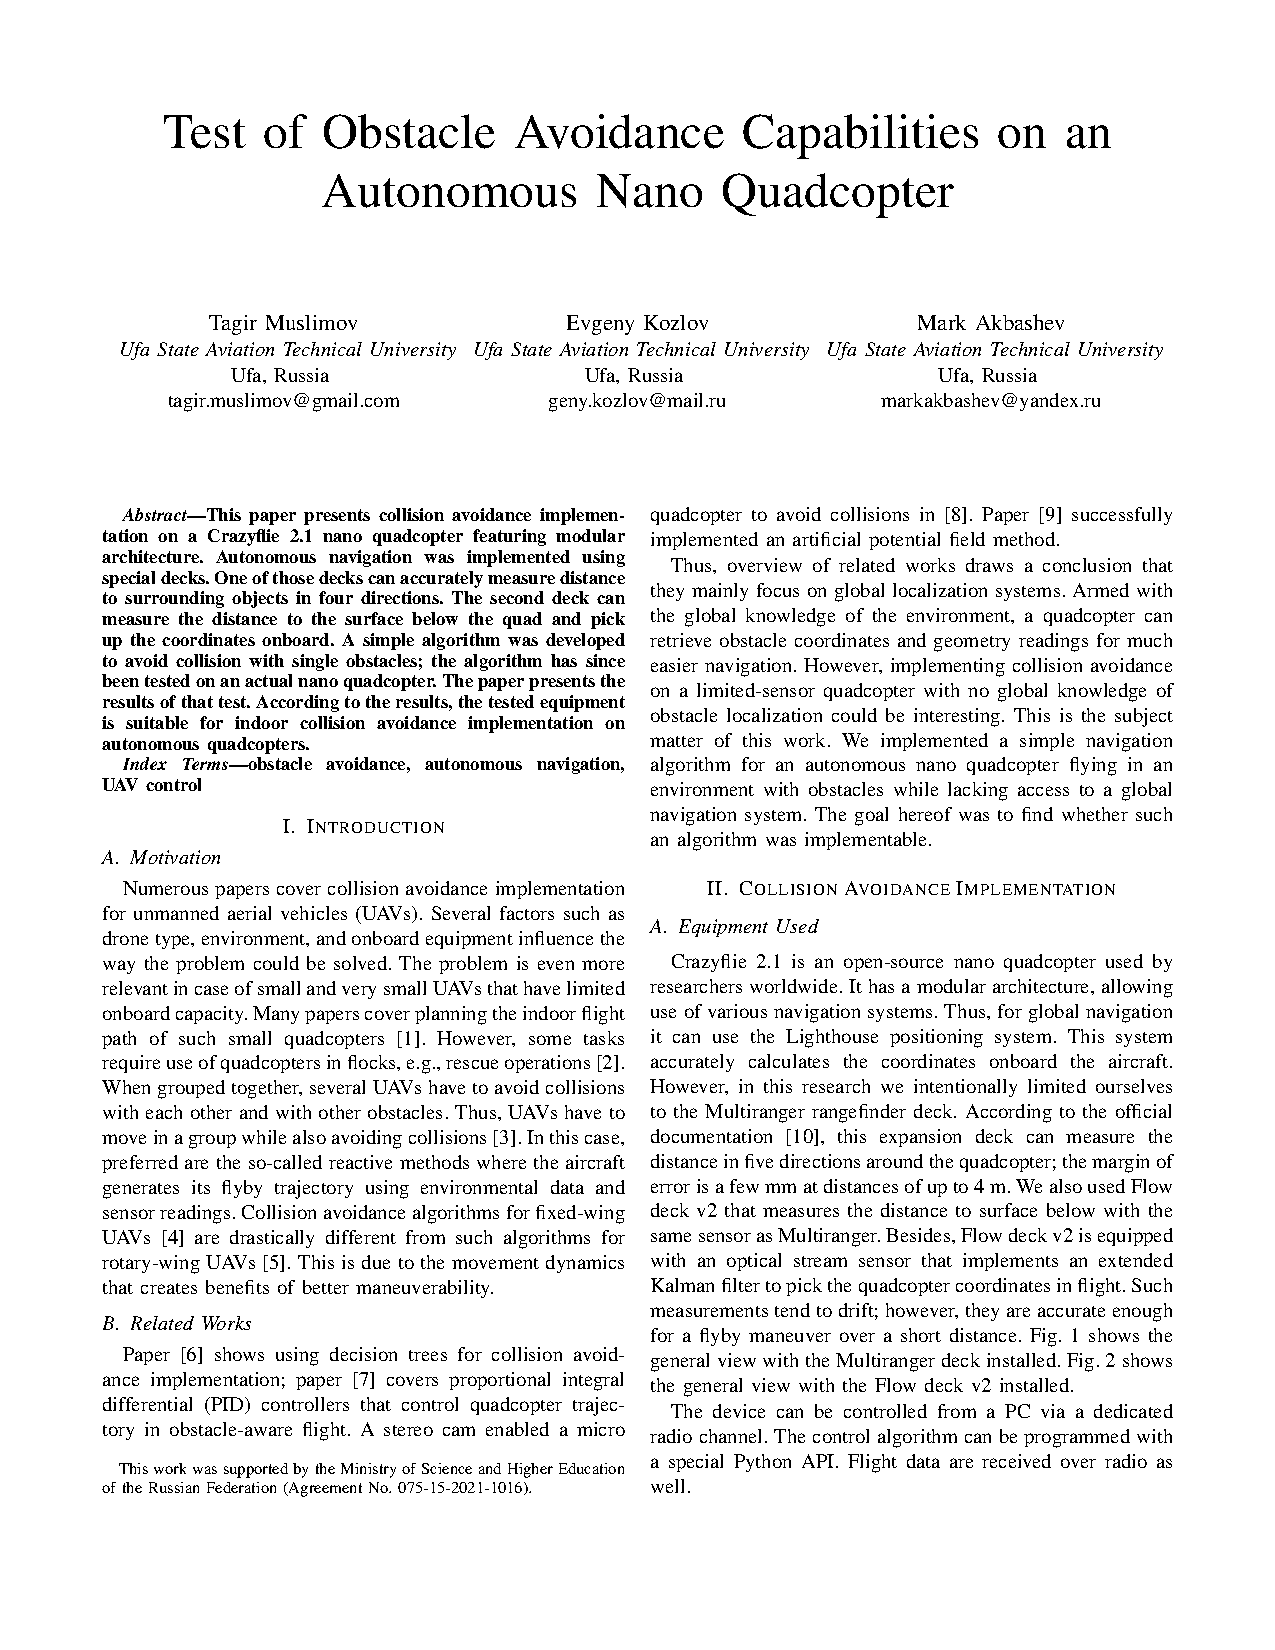
\includegraphics[width=\textwidth]{FlowDeck1}
	\end{subfigure}
	\hspace{0.01\textwidth} % Ajusta el espacio entre las imágenes
	\begin{subfigure}[b]{0.3\textwidth}
		\centering
		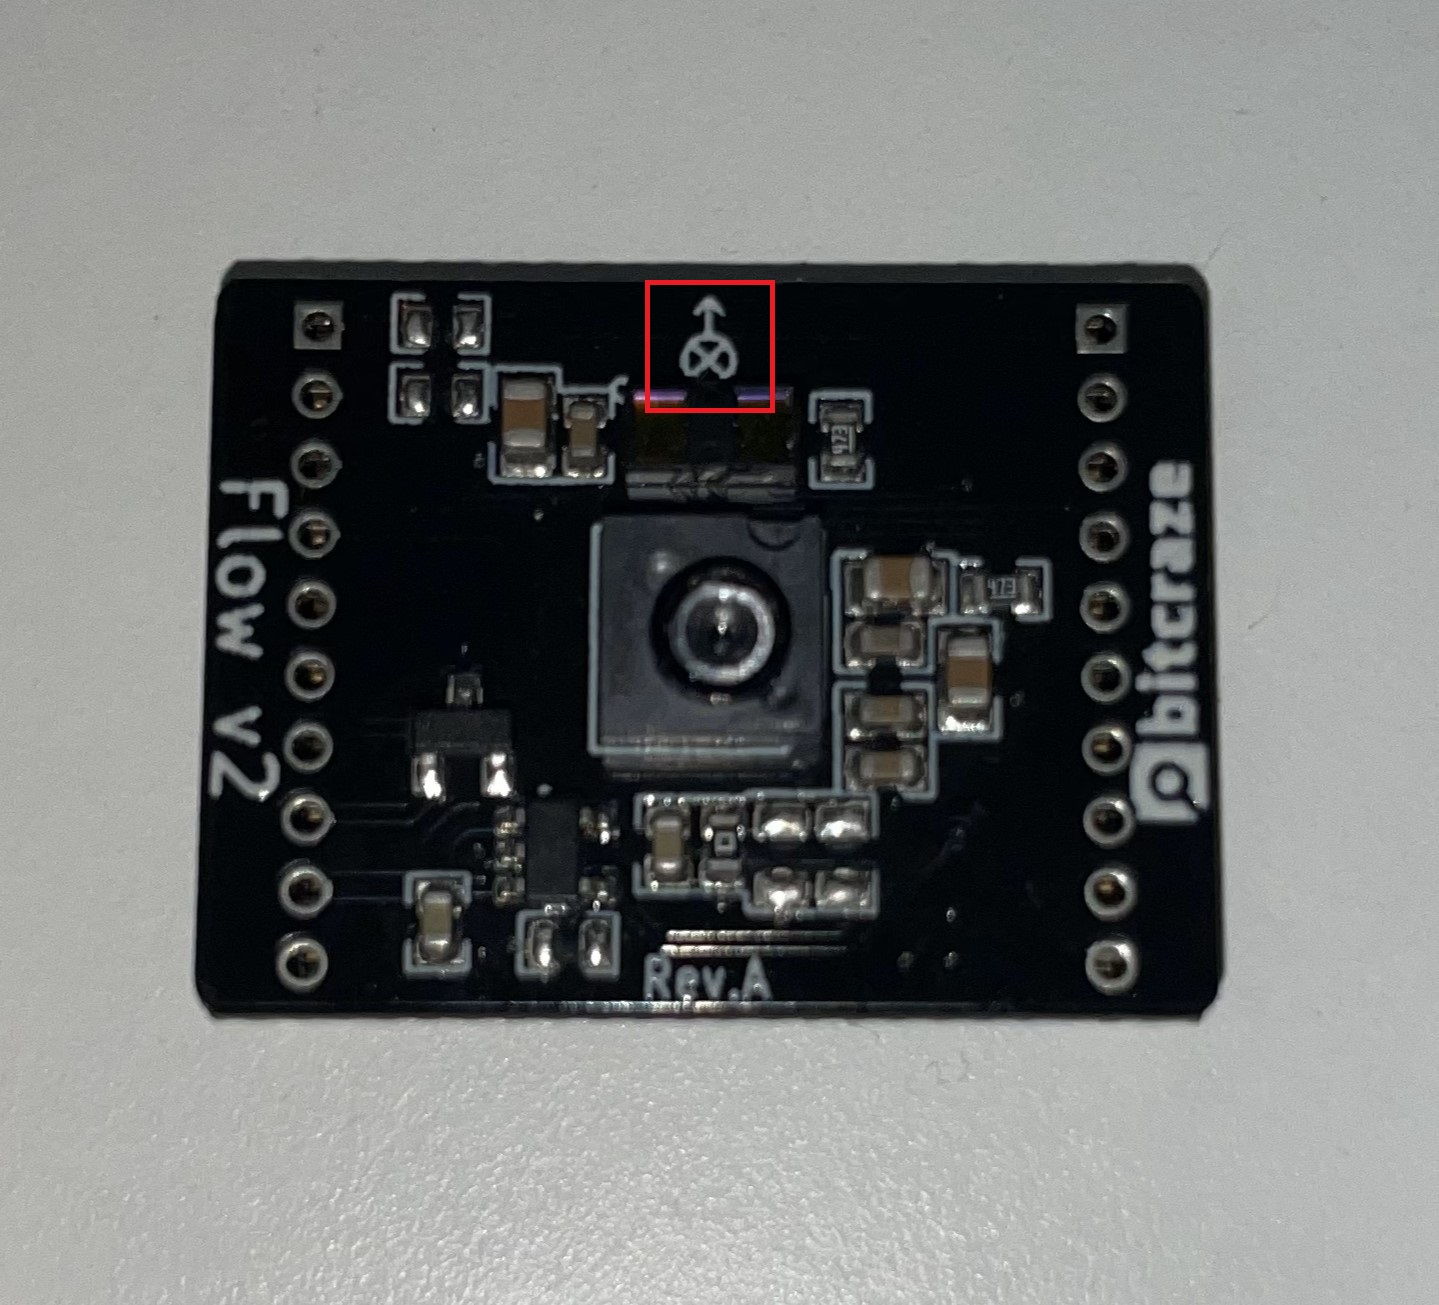
\includegraphics[width=\textwidth]{FlowDeck2}
	\end{subfigure}
	\caption{Vista frontal y trasera de la placa de expansión Flow Deck.}
	\label{fig:FlowDeck_ambas_vistas}
\end{figure}

Además de la orientación, también se debe considerar que la placa tiene una dirección específica para ser instalda. En ambas vistas de la Figura \ref{fig:FlowDeck_ambas_vistas} se observa un símbolo con un círculo y una flecha. Este mismo símbolo se encuentra en la parte inferior del Crazyflie por lo que, al momento de acoplar el sensor, es importante asegurarse que la dirección de los símbolos en ambas placas (Crazyflie y Flow Deck) coincidan, justo como se observa en la Figura \ref{fig:Crazyflie_con_FlowDeck}. De lo contrario, la placa podría experimentar daños irreversibles en el \textit{hardware}.

\begin{figure}[htbp]
	\centering
	\includegraphics[width=0.3\textwidth]{Crazyflie_con_FlowDeck2}
	\caption{Vista inferior del dron Crazyflie con la placa Flow Deck instalada.}
	\label{fig:Crazyflie_con_FlowDeck}
\end{figure} 

El siguiente aspecto que se consideró luego de instalar la placa en el dron fue la verificación de reconocimiento del sensor por parte del \textit{firmware}. Esto se realizó utilizando nuevamente el programa cfclient y conectando el Crazyflie con la placa Flow Deck instalada. 

Una vez conectado el dron al cliente, se consultó la vista de parámetros y en la sección de placas o como aparece en el cliente ``\textit{decks}'', se identificó el registro \textbf{deck.bcFlow2}. Justo como se aprecia en la Figura \ref{fig:FlowDeck_detection2}, este registro es un indicador del reconocimiento de la placa de expansión Flow Deck v2 y como este automáticamente adquirió un valor de 1 se puede asegurar que el Crazyflie detectó exitosamente al sensor.

\begin{figure}[htbp]
	\centering
	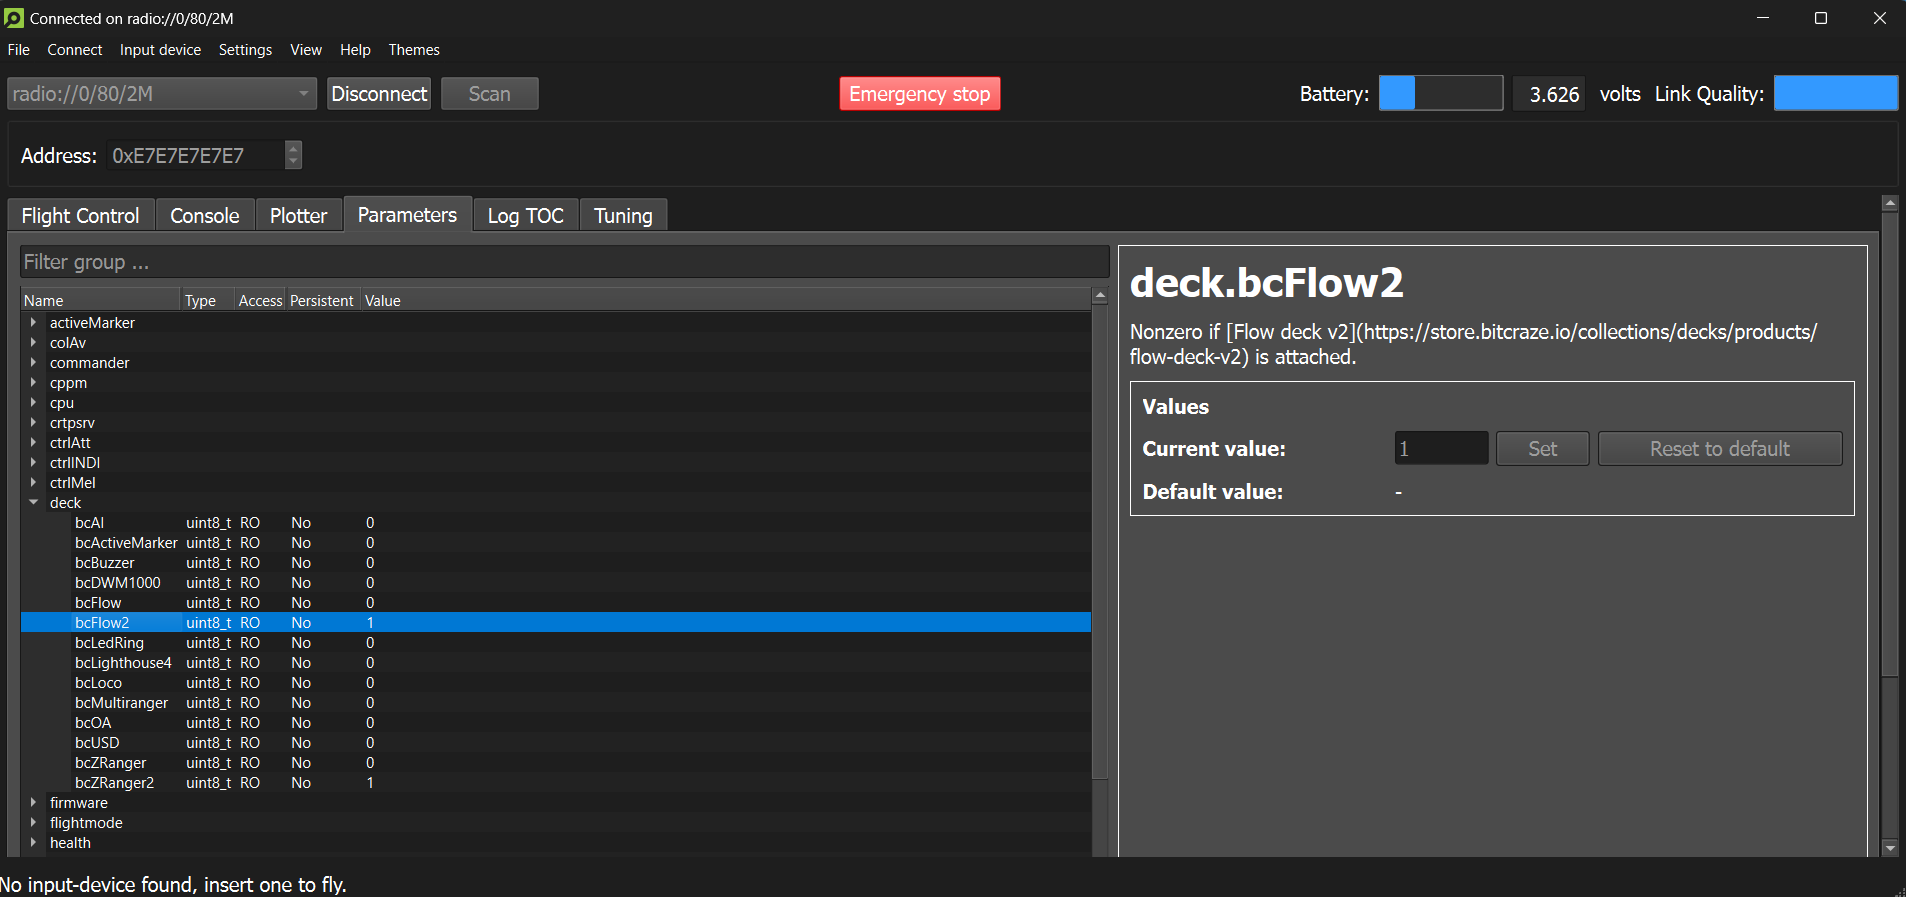
\includegraphics[width=0.85\textwidth]{FlowDeck_detection2}
	\caption{Reconocimiento de placa Flow Deck en vista de parámetros en cfclient.}
	\label{fig:FlowDeck_detection2}
\end{figure} 

Otra forma de identificar si el dron Crazyflie ha detectado a la placa Flow Deck es observar si en la vista de control de vuelo se habilitó el modo asistido flotante o bien, si se habilitaron los controles de vuelo basado en comandos (ver Figura \ref{fig:FlowDeck_detection1}). 

\begin{figure}[htbp]
	\centering
	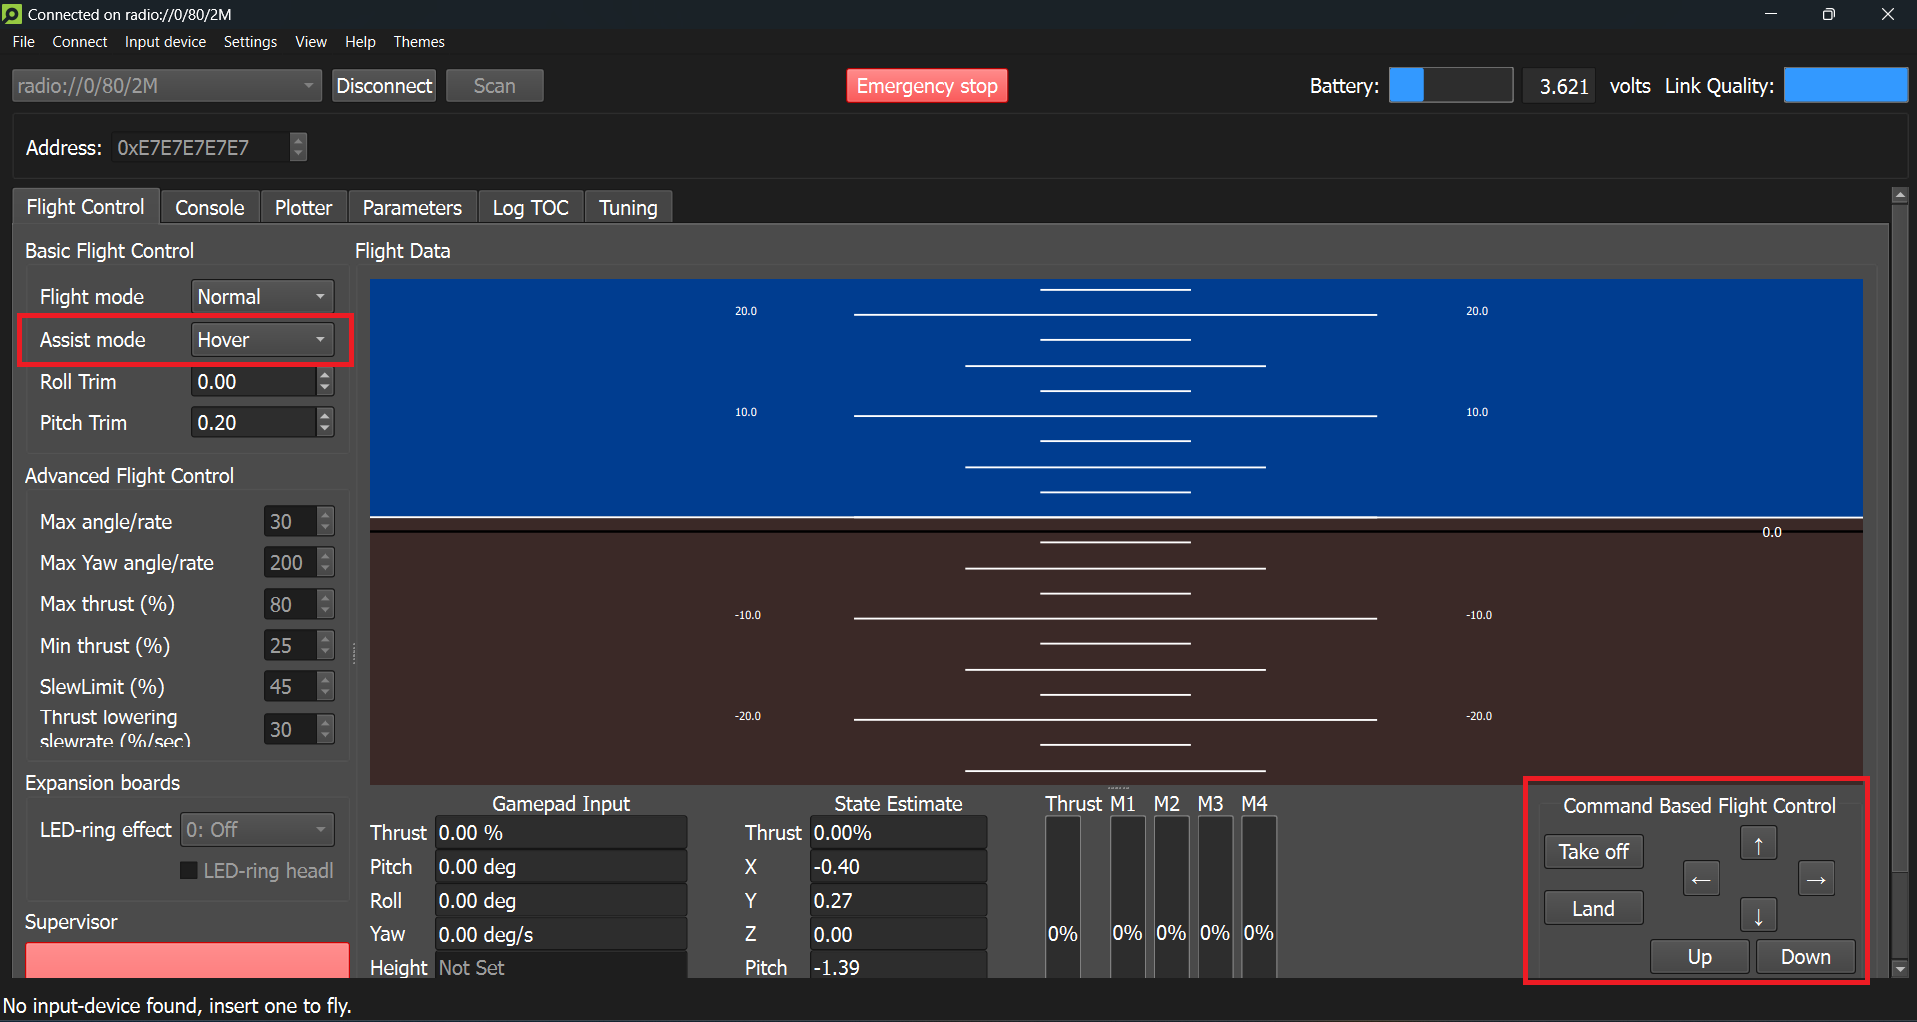
\includegraphics[width=0.85\textwidth]{FlowDeck_detection1}
	\caption{Reconocimiento de placa Flow Deck en vista de control de vuelo en cfclient.}
	\label{fig:FlowDeck_detection1}
\end{figure} 
 
\subsection{Pruebas de posicionamiento}
Luego de verificar que la placa Flow Deck había sido reconocida por el dron, se procedió a realizar pruebas de vuelo enfocadas en evaluar la mejora en el posicionamiento y estabilidad del dron. El objetivo de estas pruebas fue comparar el desempeño del Crazyflie con y sin la placa de expansión.

Tal como se realizó el experimento sin la placa, la prueba únicamente consistió en elevar el dron a cierta altura y mantenerlo levitando por algunos segundos para despues aterrizarlo. Para ello, el dron se colocó en una superficie plana y, a diferencia de las pruebas sin placa, en estas ya no fue necesario un mando pues se encontraban habilitados los controles de vuelo basados en comandos en la GUI del cfclient (como se observó en la Figura \ref{fig:FlowDeck_detection1}). Y, utilizando el comando ``\textit{take off}'' se logró despegar al dron y este mantuvo una altura constante hasta que se envió el comando ``\textit{land}'' para aterrizarlo. 

\begin{figure}[htbp]
	\centering
	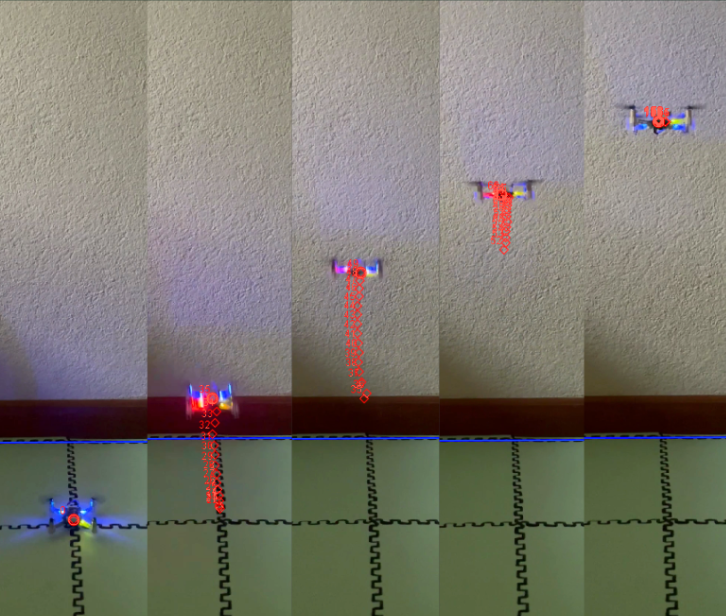
\includegraphics[width=0.5\textwidth]{Prueba_2}
	\caption{Prueba de vuelo y posicionamiento con placa Flow Deck integrada.}
	\label{fig:Prueba_2}
\end{figure} 

Justo como se observa en la Figura anterior \ref{fig:Prueba_2}, el desempeño de vuelo del dron es significativamente mejor que el obtenido para la misma prueba pero sin la placa de posicionamiento. Validando su instalación y reconocmiento en el \textit{firmware} del dron.
 
 
\section{Adaptación de entorno}
Al realizar las pruebas de posicionamiento con la placa Flow Deck, se observó que para distintas condiciones del entorno y para diferentes superficies el comportamiento de posicionamiento del dron Crazyflie fue variable. Esto se debió a las características de los sensores en la placa que mejoran funcionamiento en condiciones específicas. Por ello, surgió la necesidad de identificar un entorno de pruebas con las condiciones óptimas para el correcto desempeño de la placa Flow Deck. 

\subsection{Superficies y condiciones desfavorables}
Durante las pruebas realizadas, se observaron dificultades en la capacidad del dron para mantener su posición cuando se encontraba volando sobre superficies con condiciones de alta reflectividad, demasiada homogeneidad y con condiciones de luz intensas. 
\begin{itemize} 
	\item La homogeneidad en las superficies representó un problema en el desempeño del dron debido a que el sensor de flujo óptico de la placa no era capaz de interpretar movimiento relativo al no identificar diferencias significativas en las imágenes de la superficie.
	\item La condición de luz intensa con sombras muy marcadas también afectó al sensor de flujo óptico, ya que la propia sombra del dron sobre la superficie generaba errores en el cálculo de movimiento relativo.
	\item La reflectividad en las superficies perjudicó el funcionamiento del sensor infrarrojo de la placa, provocando que esta no determinara correctamente el movimiento relativo por no tener una lectura correcta de la posición vertical del dron.
\end{itemize}

\vspace{0.7cm}

\begin{figure}[htbp]
	\centering
	\begin{subfigure}[b]{0.26\textwidth}
		\centering
		\includegraphics[width=\textwidth]{superficie1}
	\end{subfigure}
	\hspace{0.01\textwidth} % Ajusta el espacio entre las imágenes
	\begin{subfigure}[b]{0.26\textwidth}
		\centering
		\includegraphics[width=\textwidth]{superficie2}
	\end{subfigure}
	\label{fig:Superficies_probadas1}
\end{figure}

\begin{figure}[htbp]
	\centering
	\begin{subfigure}[b]{0.26\textwidth}
		\centering
		\includegraphics[width=\textwidth]{superficie3}
	\end{subfigure}
	\hspace{0.01\textwidth} % Ajusta el espacio entre las imágenes
	\begin{subfigure}[b]{0.27\textwidth}
		\centering
		\includegraphics[width=\textwidth]{superficie4}
	\end{subfigure}
	\caption{Superficies de prueba con pésimos resultados debido a condiciones anteriormente descritas.}
	\label{fig:Superficies_probadas2}
\end{figure}

En la Figura \ref{fig:Superficies_probadas2} se muestran algunas de las superficies que fueron probadas. La primer imagen es en la superficie natural del ecosistema Robotat, pero la homogeneidad de la superficie presentó un pésimo posicionamiento, provocando que el dron volara erráticamente. La segunda y tercera figura corresponden a papel mate con patrones impresos sin embargo, la pintura utilizada presentó alta reflectividad, lo que produjo que el dron no fuera capaz de estimar correctamente su posición. La última superficie, una alfombra con cubierta impresa de grama artificial presento el mismo problema debido a ser muy reflectiva.

\subsection{Solución de entorno y observaciones}
Para mitigar los problemas de funcionamiento debido a las condiciones del entorno, se tomaron varias medidas. Primero, se ajustó el entorno de vuelo empleando una superficie antirreflejante con patrones visibles, lo que mejoró significativamente la capacidad de los sensores del Flow Deck. Las superficies antirreflejantes utilizadas consistieron en alfombras modulares de foami con patrones situados con pintura antireflejante, justo como se observa en la Figura \ref{fig:Superficie_funcional_1}.  

\vspace{0.25cm}
\begin{figure}[htbp]
	\centering
	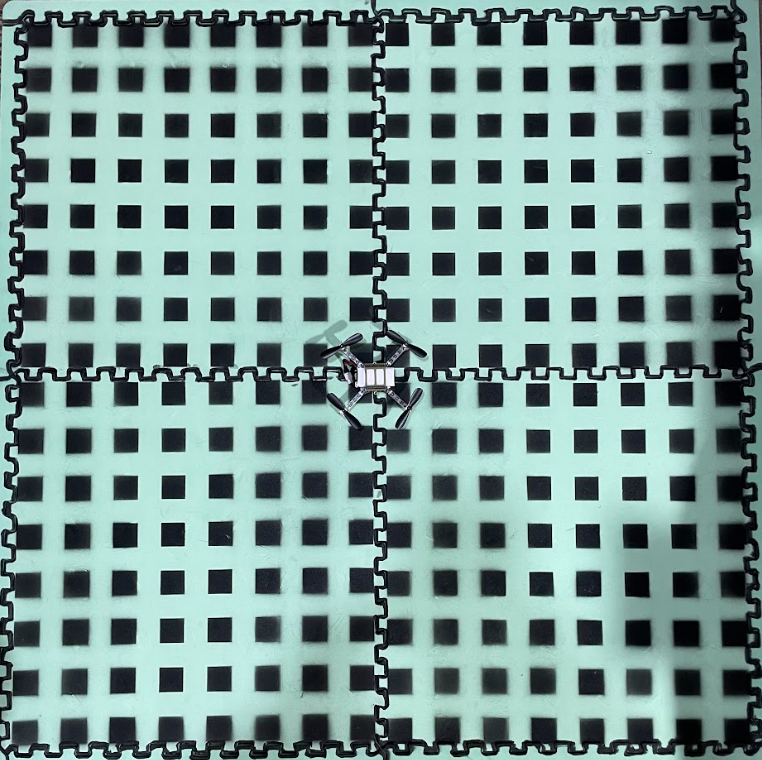
\includegraphics[width=0.6\textwidth]{superficie5}
	\caption{Prototipo de superficie adaptada para el funcionamiento de la placa Flow Deck.}
	\label{fig:Superficie_funcional_1}
\end{figure} 

Estas alfombras pueden ser adaptadas en distintos entornos y resultan especialmente prácticas para ser instaladas en el ecositema Robotat, pues pueden ser colocadas y retiradas con facilidad. Además, al ser de material foami tienen la característica de ser amortiguadoras, ayudando a reducir el daño en el \textit{hardware} del dron en caso de colisiones por fallas o errores.

Otro aspececto importante que se tuvo en consideración fue la ilumincación del entorno. Fue importante asegurarse que la distribución de luz sea adecuada, de forma que se minimice al máximo la propia sombra del dron y para que no termine afectando a las lecturas del sensor de flujo óptico.

Estas mejoras permitieron un rendimiento más estable del dron, asegurando que el Flow Deck pudiera operar de manera óptima. Estas observaciones son fundamentales para futuros experimentos, recomendando realizar vuelos en entornos controlados y adecuadamente preparados para evitar problemas de posicionamiento. 


% ------------------------------------------------------------------------------
% CAPÍTULO 8 -------------------------------------------------------------------
% ------------------------------------------------------------------------------
\chapter{Herramientas de software para control individual de dron Crazyflie}
En este capítulo se presenta el desarrollo e implementación de algoritmos de control básicos para el dron Crazyflie con la placa Flow Deck integrada. Se detallan los pasos de instalación de las dependencias, desarrollo de funciones de control específicas en Python y su implementación desde el entorno de Matlab. Además, se presenta un método para mejorar el rendimiento de vuelo al mezclar las lecturas de posicionamiento de la placa Flow Deck con lecturas de un sistema de captura de movimiento. Por último, se presentan herramientas de simulación para experimentar con el dron Crazyflie, detallando los alcances de estas. 

\section{Algoritmos de control básico en Python}
Con el fin de lograr un control efectivo del dron Crazyflie, se desarrollaron una serie de algoritmos básicos en Python utilizando la librería oficial de Crazyflie en python, cflib. Estos algoritmos permiten ejecutar comandos para conexión, lectura de variables, configuración de parámetros y movimiento básicos de vuelo. Estas proporcionan una base para realizar una amplia variedad de experimentos.

\subsection{Instalación de librería cflib}
La librería Crazyflie es una herramienta fundamental para interactuar y controlar al dron mediante algoritmos en Python. Para su instalación es necesario asegurarse previamente de tener instalada una versión de Python entre las versiones 3.7 y 3.11. Para el desarrollo del proyecto se instaló la versión 3.11.0 disponible para Windows 11 en la página oficial de Python \cite{Python_3_11_0}. Al instalarlo se tomó el cuidado de asegurarse que la ruta a Python estuviera agregada al PATH.

\newpage
Para confirmar la versión de Python instalada en el sistema, se ejecuta el siguiente comando en la terminal de Windows:

\begin{verbatim}
	python --version
\end{verbatim}

El resultado en consola confirma que la versión en uso es la \textbf{3.11.0}, como se muestra en la Figura \ref{fig:cmd_python_version}.

Una vez verificada la versión de Python, se procede a la instalación de cflib mediante el gestor de paquetes pip, ejecutando el siguiente comando:

\begin{verbatim}
	pip install cflib
\end{verbatim}

Al ejecutar este comando, se descargan e instalan automáticamente las dependencias necesarias, como \textbf{pyusb}, \textbf{libusb-package}, \textbf{scipy}, \textbf{numpy}, entre otras. La versión de la librería instalada fue \textbf{cflib-0.1.26}, como se observa en la Figura \ref{fig:cmd_python_version}.

\vspace{0.5cm}
\begin{figure}[htbp]
	\centering
	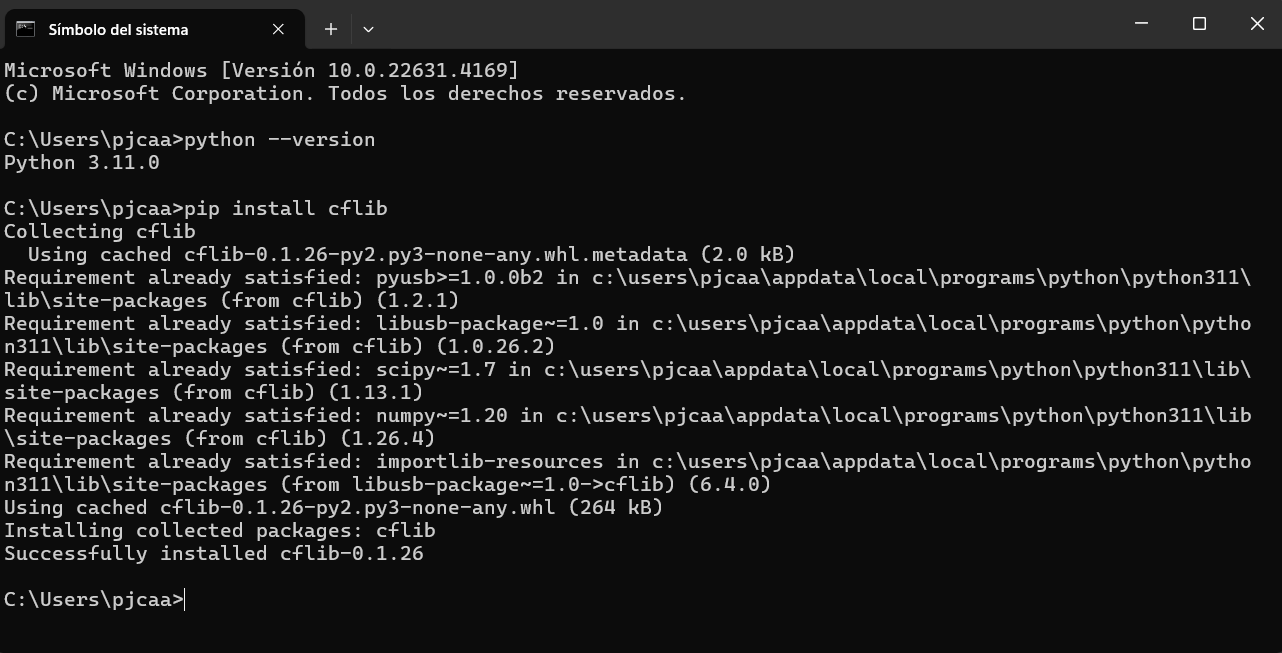
\includegraphics[width=0.9\textwidth]{cmd_python_version}
	\caption{Ejecución de comandos en la terminal de Windows.}
	\label{fig:cmd_python_version}
\end{figure} 
\vspace{0.5cm}

Tras la instalación, se llevaron a cabo pruebas básicas para garantizar que la librería cflib se instaló correctamente y que el dron puede recibir comandos desde un script de Python. Es importante mencionar que, a lo largo de este proyecto se utilizó el programa \textit{Visual Studio Code} como editor de texto para los algoritmos en Python. 

A continuación, se presenta el código de prueba que realiza la conexión y desconexión del dron (ver Código \ref{code:prueba_conexion_crazyflie}). 

\newpage
\begin{lstlisting}[caption=Algoritmo de prueba en Python utilizando la librería Cflib., label=code:prueba_conexion_crazyflie]
	import time
	import cflib.crtp
	from cflib.crazyflie import Crazyflie
	
	# Inicializar los drivers
	cflib.crtp.init_drivers()
	
	# Crear el objeto Crazyflie
	cf = Crazyflie(rw_cache='./cache')
	
	try:
		# Intentar conectar al Crazyflie
		cf.open_link('radio://0/80/2M/E7E7E7E7E7')
		print("Crazyflie conectado.")
		time.sleep(5)  # Espera 5 segundos
	except Exception as e:
		print(f"Ocurrió un error al intentar la conexión: {e}")
	finally:
		# Asegurar la desconexión del Crazyflie
		cf.close_link()
		print("Crazyflie desconectado.")
\end{lstlisting}

El algoritmo presentado realiza un proceso simple de conexión con el dron Crazyflie, manteniendo activa la conexión por 5 segundos para luego cerrar la conexión. Para lograrlo se utilizó la libería time y los módulos CRTP y Crazyflie de la libería cflib. El móudlo CRTP se utilizó para inicializar los drivers para el dispositivo Crazyradio y el módulo Crazyflie se empleó para instanciar un objeto de la clase princial Crazyflie, este fue la representación del dron en el código. En la Figura \ref{fig:algoritmo_prueba_vs}, se muestra el entorno de desarrollo de \textit{VS Code} y la correcta compilación y ejecución del algoritmo de prueba. 

\begin{figure}[htbp]
	\centering
	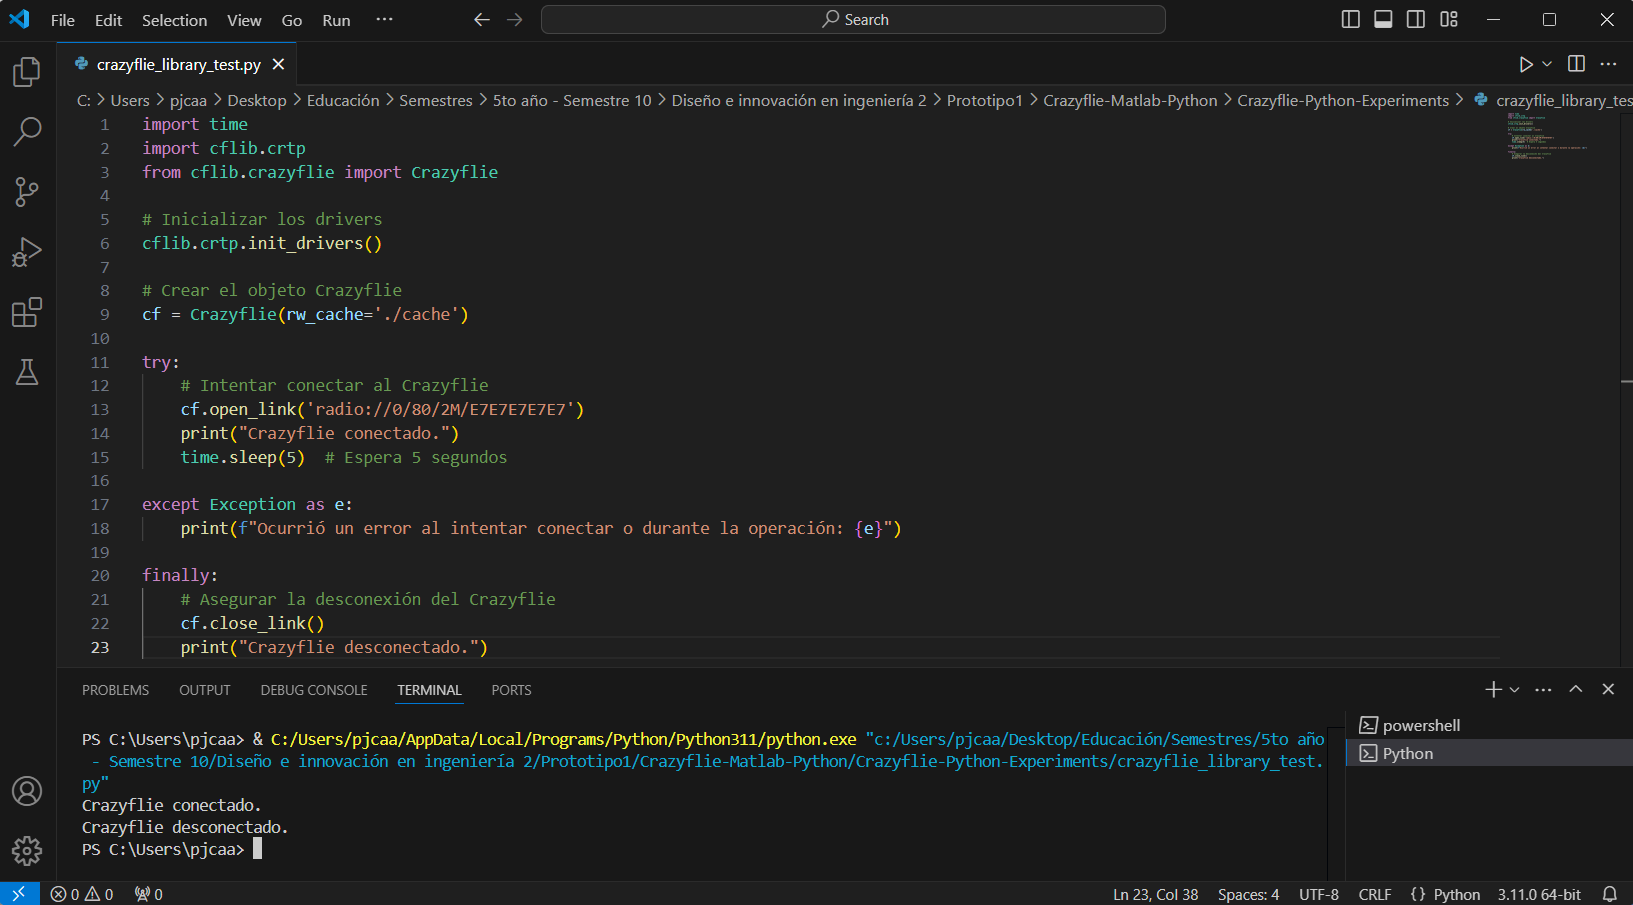
\includegraphics[width=1\textwidth]{algoritmo_prueba_vs}
	\caption{Ejecución de algoritmo de prueba en \textit{Visual Studio Code}.}
	\label{fig:algoritmo_prueba_vs}
\end{figure}

\newpage
\subsection{Uso de librería cflib y recursos adicionales}
Para el desarrollo de los algoritmos de control se utilizaron módulos específicos de la librería cflib para Crazyflie y algunas librerías estándar de python. A continuación, se detallan las librerías y módulos utilizados y su propósito:

\subsubsection{Módulos de cflib utilizados}

\begin{itemize}
	\item \textbf{CRTP:} El módulo cflib.crtp es responsable de inicializar los drivers necesarios para la comunicación mediante el protocolo \textit{Crazy Real-Time Protocol}, utilizado para establecer la conexión con el dron a través del dispositivo Crazyradio.
	\item \textbf{Crazyflie:} El módulo cflib.crazyflie es la interfaz que permite controlar y comunicarse con el dron. 
	\begin{itemize}
		\item Submódulo Log: El submódulo cflib.crazyflie.log se empleó para configurar los registros de variables en tiempo real.
		\item Submódulo SyncCrazyflie: El submódulo cflib.crazyflie.synccrazyflie se empleó para simplificar el manejo de conexiones mediante el uso de la subclase SyncCrazyflie. 
		\item Submódulo HighLevelCommander: El submódulo cflib.crazyflie.high\_level\_commander se empleó como una interfaz de alto nivel para el envío de comandos de control de vuelo hacia el dron. 
	\end{itemize}
\end{itemize} 

Es importante mencionar que se utilizó la versión síncrona de la librería Crazyflie en lugar de la versión asíncrona, como se evidencia en el uso de la subclase SyncCrazyflie. Esta convierte a las funciones no bloqueantes de la versión asíncrona en funciones bloqueantes, lo que significa que el programa espera a que una tarea termine antes de continuar con la siguiente.

Esta elección se realizó por la necesidad de ejecutar comandos de control de manera secuencial y confiable. Al utilizar una versión síncrona, se asegura que cada acción enviada sea completada antes de ejecutar la siguiente. De esta forma el dron puede completar algoritmos de forma secuencial, tal como se esperaría para un algoritmo de seguimiento de trayectorias.

\subsubsection{Recursos adicionales de Python utilizados}
\begin{itemize}
	\item \textbf{logging:} Se utilizó para configurar el nivel de registro de mensajes dentro del programa. 
	\item \textbf{time:} Se utilizó para realizar gestión de tiempo en la ejecución de las funciones de control. Esto asegurpo que el dron tuviera el tiempo suficiente para ejecutar las acciones solicitadas previo al siguiente comando.
	\item \textbf{sys:} Se utilizó para forzar la salida inmediata de los mensajes en la consola. Esto evitó que el sistema almacenara mensajes en \textit{buffer} y retrasara su impresión en consola.
	\item \textbf{threading:} Se utilizó la clase \textit{Event} del módulo para sincronizar la recepción de datos del dron.
\end{itemize} 

\subsection{Desarrollo de algoritmos de control}
A continuación, se presentan las funciones desarrolladas en python con algoritmos de control de funcionalidades básicas del dron Crazyflie. Están clasificadas en cuatro grupos: conexión, lectura de variables, configuración de parámetros y movimiento general.

\subsubsection{Funciones de conexión}
\begin{itemize}
	\item \textbf{connect(uri)} \ref{code:funcion_connect} \\ 
	Esta función se utiliza para establecer y mantener una conexión activa con el dron Crazyflie de manera síncrona. Requiere que sea especificado el Identificador Unifrome de Recursos (URI) del Crazyflie objetivo . 
	\begin{itemize}
		\item Atributos:
		\begin{itemize}
			\item \texttt{uri} (\texttt{str}): Dirección URI del Crazyflie a conectar.
		\end{itemize}
		\item Valor de retorno:
		\begin{itemize}
			\item Retorna una instancia de la clase \texttt{SyncCrazyflie} si la conexión es exitosa.
			\item Imprime en consola un mensaje de confirmación de conexión o de alerta de error con los detalles correspondientes.
		\end{itemize}
	\end{itemize} 

	\item \textbf{disconnect(SyncCrazyflie)} \ref{code:funcion_disconnect} \\ 
	Esta función se utiliza para cerrar la conexión activa con el dron Crazyflie. Requiere que sea especificada la instancia de la clase \texttt{SyncCrazyflie} generada al conectarse . 
	\begin{itemize}
		\item Atributos:
		\begin{itemize}
			\item \texttt{SyncCrazyflie} (\texttt{scf}): Instancia de la clase \texttt{SyncCrazyflie} generada al establecer la conexión.
		\end{itemize}
		\item Valor de retorno:
		\begin{itemize}
			\item Imprime en consola un mensaje de confirmación de desconexión o de alerta de error con los detalles correspondientes.
		\end{itemize}
	\end{itemize} 
\end{itemize}

\subsubsection{Funciones de lectura de variables}
\begin{itemize}
	\item \textbf{get\_pose(SyncCrazyflie)} \ref{code:funcion_get_pose}\\ 
	Esta función se utiliza para obtener los valores actuales de los registros de la estimación de posición del dron Crazyflie.
	\begin{itemize}
		\item Atributos:
		\begin{itemize}
			\item \texttt{SyncCrazyflie} (\texttt{scf}): Instancia de la clase \texttt{SyncCrazyflie} generada al establecer la conexión.
		\end{itemize}
		\item Valor de retorno:
		\begin{itemize}
			\item Retorna un diccionario con los valores de posición actuales del Crazyflie. Las llaves del diccionario correspondiente son: 'x', 'y', 'z', 'roll', 'pitch', 'yaw'.
			\item Imprime en consola un mensaje con los valores de posición actual o un mensaje de alerta de error con los detalles correspondientes.
		\end{itemize}
	\end{itemize} 
	\vspace{1mm} % Espacio adicional entre funciones
	\item \textbf{get\_pid\_values(SyncCrazyflie)} \ref{code:funcion_get_pid_values}\\ 
	Esta función se utiliza para obtener los valores actuales de los registros de los controladores PID de posición del Crazyflie.
	\begin{itemize}
		\item Atributos:
		\begin{itemize}
			\item \texttt{SyncCrazyflie} (\texttt{scf}): Instancia de la clase \texttt{SyncCrazyflie} generada al establecer la conexión.
		\end{itemize}
		\item Valor de retorno:
		\begin{itemize}
			\item Retorna un diccionario con los valores actuales de los controladores PID de posición  del Crazyflie. Las llaves del diccionario correspondiente son: 'X', 'Y', 'Z' y cada una posee un arreglo con las constantes P, I y D.
			\item Imprime en consola un mensaje con los valores actuales de los controladores PID de posición o un mensaje de alerta de error con los detalles correspondientes.
		\end{itemize}
	\end{itemize} 
	\vspace{1mm} % Espacio adicional entre funciones
	
	\item \textbf{get\_pid\_x(scf)}, \textbf{get\_pid\_y(scf)} y \textbf{get\_pid\_z(scf)} \ref{code:funcion_get_pid_x}\\
	Estas funcones se utilizan para obtener los valores actuales del controlador PID de posición en el eje correspondiente del dron Crazyflie.
	\begin{itemize}
		\item Atributos:
		\begin{itemize}
			\item \texttt{SyncCrazyflie} (\texttt{scf}): Instancia de la clase \texttt{SyncCrazyflie} generada al establecer la conexión.
		\end{itemize}
		\item Valor de retorno:
		\begin{itemize}
			\item Retorna un arreglo con los valores actuales de las tres constantes del controlador PID de posición del eje correspondiente.
			\item Imprime en consola un mensaje con los valores del controlador PID de posición del eje correspondiente o un mensaje de alerta de error con los detalles correspondientes.
		\end{itemize}
	\end{itemize}
	\vspace{1mm} % Espacio adicional entre funciones
	
	\item \textbf{detect\_flow\_deck(SyncCrazyflie)} \ref{code:funcion_detect_flow_deck}\\ 
	Esta función se utiliza verificar que el dron Crazyflie conectado esté detectando correctamente a la placa de expansión Flow Deck. Fue desarrollada como una función de prevención de accidentes, ya que si no se detecta dicha placa el comportamiento del dron Crazyflie es errático. 
	\begin{itemize}
		\item Atributos:
		\begin{itemize}
			\item \texttt{SyncCrazyflie} (\texttt{scf}): Instancia de la clase \texttt{SyncCrazyflie} generada al establecer la conexión.
		\end{itemize}
		\item Valor de retorno:
		\begin{itemize}
			\item Retorna un valor True si se detecta correctamente la placa Flow Deck y False si esta no es detectada. 
			\item Imprime en consola un mensaje confimando o negando la detección de la placa de expansión Flow Deck.
		\end{itemize}
	\end{itemize} 
	\vspace{5mm} % Espacio adicional entre funciones 
\end{itemize}

\subsubsection{Funciones de configuración de parámetros}
\begin{itemize}
	\item \textbf{set\_position(SyncCrazyflie, x, y, z)} \ref{code:funcion_set_position}\\ 
	Esta función se utiliza para configurar el valor en los registros de la estimación de posición del dron Crazyflie. Es decir, actualiza la posición actual en el marco de referencia relativo del dron Crazyflie.
	\begin{itemize}
		\item Atributos:
		\begin{itemize}
			\item \texttt{SyncCrazyflie} (\texttt{scf}): Instancia de la clase \texttt{SyncCrazyflie} generada al establecer la conexión.
			\item \texttt{x} (\texttt{float}): Coordenada X en metros de la posición a configurar.
			\item \texttt{y} (\texttt{float}): Coordenada Y en metros de la posición a configurar.
			\item \texttt{z} (\texttt{float}): Coordenada Z en metros de la posición a configurar.
		\end{itemize}
		\item Valor de retorno:
		\begin{itemize}
			\item Imprime en consola un mensaje de confirmación de actualización de posición relativa o un mensaje de alerta de error con los detalles correspondientes.
		\end{itemize}
	\end{itemize} 
	\vspace{1mm} % Espacio adicional entre funciones
	
	\item \textbf{set\_pid\_values(SyncCrazyflie, p\_gains, i\_gains, d\_gains)} \ref{code:funcion_set_pid_values}\\ 
	Esta función se utiliza para configurar los valores actuales de los registros de los controladores PID de posición del Crazyflie.
	\begin{itemize}
		\item Atributos:
		\begin{itemize}
			\item \texttt{SyncCrazyflie} (\texttt{scf}): Instancia de la clase \texttt{SyncCrazyflie} generada al establecer la conexión.
			\item \texttt{p\_gains} (\texttt{diccionario}): Diccionario con constantes proporcionales de los controladores PID de posición para los ejes XYZ. Las llaves del diccionario deben ser: 'X', 'Y' y 'Z'.
			\item \texttt{i\_gains} (\texttt{diccionario}): Diccionario con constantes integrativas de los controladores PID de posición para los ejes XYZ. Las llaves del diccionario deben ser: 'X', 'Y' y 'Z'.
			\item \texttt{d\_gains} (\texttt{diccionario}): Diccionario con constantes derivativas de los controladores PID de posición para los ejes XYZ. Las llaves del diccionario deben ser: 'X', 'Y' y 'Z'.
		\end{itemize}
		\item Valor de retorno:
		\begin{itemize}
			\item Imprime en consola un mensaje de confirmación de actualización de constantes de controladores PID de posición o un mensaje de alerta de error con los detalles correspondientes.
		\end{itemize}
	\end{itemize} 
	\vspace{1mm} % Espacio adicional entre funciones
	
	\item \textbf{set\_pid\_x(scf, P, I, D)}, \textbf{set\_pid\_y(scf, P, I, D)} y \textbf{set\_pid\_z(scf, P, I, D)} \ref{code:funcion_set_pid_x} \\
	Estas funciones se utilizan para configurar los valores de las constantes del controlador PID de posición en el eje correspondiente del dron Crazyflie.
	\begin{itemize}
		\item Atributos:
		\begin{itemize}
			\item \texttt{SyncCrazyflie} (\texttt{scf}): Instancia de la clase \texttt{SyncCrazyflie} generada al establecer la conexión.
			\item \texttt{P} (\texttt{float}): Constante proporcional para el controlador PID de posición del eje correspondiente.
			\item \texttt{I} (\texttt{float}): Constante integrativa para el controlador PID de posición del eje correspondiente.
			\item \texttt{D} (\texttt{float}): Constante derivativa para el controlador PID de posición del eje correspondiente.
		\end{itemize}
		\item Valor de retorno:
		\begin{itemize}
			\item Imprime en consola un mensaje con los valores del controlador PID de posición del eje correspondiente o un mensaje de alerta de error con los detalles correspondientes.
		\end{itemize}
	\end{itemize} 
\end{itemize}

\subsubsection{Funciones de movimiento}
\begin{itemize}
		\item \textbf{takeoff(SyncCrazyflie, height, duration)} \ref{code:funcion_takeoff}\\ 
	Esta función se utiliza para realizar el despegue del dron Crazyflie a una altura dada durante una duración especificada. En caso de no ser especificados la altura y duración, se utilizan los valores por defecto de 0.3 metros y 1 segundo.
	\begin{itemize}
		\item Atributos:
		\begin{itemize}
			\item \texttt{SyncCrazyflie} (\texttt{scf}): Instancia de la clase \texttt{SyncCrazyflie} generada al establecer la conexión.
			\item \texttt{height} (\texttt{float}): Altura en metros que alcanzará durante el despegue. 
			\item \texttt{duration} (\texttt{float}): Tiempo en segundos que tardará en alcanzar la altura de despegue indicada.
		\end{itemize}
		\item Valor de retorno:
		\begin{itemize}
			\item Imprime en consola un mensaje de confirmación de despegue completado o de alerta de error con los detalles correspondientes.
		\end{itemize}
	\end{itemize} 
	\vspace{5mm} % Espacio adicional entre funciones
	
	\item \textbf{land(SyncCrazyflie, height, duration)} \ref{code:funcion_land}\\ 
	Esta función se utiliza para realizar el aterrizaje del dron Crazyflie a una altura dada durante una duración especificada. En caso de no ser especificados la altura y duración, se utilizan los valores por defecto de 0 metros y 2 segundos.
	\begin{itemize}
		\item Atributos:
		\begin{itemize}
			\item \texttt{SyncCrazyflie} (\texttt{scf}): Instancia de la clase \texttt{SyncCrazyflie} generada al establecer la conexión.
			\item \texttt{height} (\texttt{float}): Altura en metros que alcanzará durante el despegue. 
			\item \texttt{duration} (\texttt{float}): Tiempo en segundos que tardará en alcanzar la altura de aterrizaje indicada.
		\end{itemize}
		\item Valor de retorno:
		\begin{itemize}
			\item Imprime en consola un mensaje de confirmación de aterrizaje completado o de alerta de error con los detalles correspondientes.
		\end{itemize}
	\end{itemize} 
	\vspace{5mm} % Espacio adicional entre funciones
	
	\item \textbf{move\_to\_position(SyncCrazyflie, x, y, z, velocity)} \ref{code:funcion_move_to_position}\\ 
	Esta función se utiliza para mover al dron a una posición nueva con una velocidad dada. Requiere de las coordenadas XYZ de la nueva posición y la velocidad del movimiento. La velocidad puede ser omitida y toma el valor por defecto de 1 metro por segundo. 
	\begin{itemize}
		\item Atributos:
		\begin{itemize}
			\item \texttt{SyncCrazyflie} (\texttt{scf}): Instancia de la clase \texttt{SyncCrazyflie} generada al establecer la conexión.
			\item \texttt{x} (\texttt{float}): Coordenada X en metros de la nueva posición.
			\item \texttt{y} (\texttt{float}): Coordenada Y en metros de la nueva posición.
			\item \texttt{z} (\texttt{float}): Coordenada Z en metros de la nueva posición.
			\item \texttt{velocity} (\texttt{float}):Velocidad en metros por segundo del movimiento.
		\end{itemize}
		\item Valor de retorno:
		\begin{itemize}
			\item Imprime en consola un mensaje de confirmación de posición alcanzada o de alerta de error con los detalles correspondientes.
		\end{itemize}
	\end{itemize} 
\end{itemize}

\subsection{Experimentos con algoritmos de control}
Una vez desarrollados los algoritmos de control básicos en forma de funciones de Python, se desarrollaron algoritmos utilizando dichas funciones para validar su uso en experimentos simples. Se realizaron tres experimentos: prueba de despegue simple \ref{code:python_prueba1}, prueba de despegue y aterrizaje con modificación del PID de posición z \ref{code:python_prueba2} y prueba movimiento de punto a punto \ref{code:python_prueba3}.

\subsubsection{Experimento simple de despegue y aterrizaje}
\vspace{2mm} % Espacio adicional entre funciones
\begin{lstlisting}[caption=Algoritmo de prueba de takeoff y land con Crazyflie., label=code:python_prueba1]
	def main():
		uri = 'radio://0/80/2M/E7E7E7E7E7'
		scf = connect(uri)
		
		if scf:
			takeoff(scf, height=0.5, duration=3.0)  
			land(scf, height=0.0, duration=2.0)     
			disconnect(scf)  
		else:
			print("Failed to establish a connection to the Crazyflie.")
	
	if __name__ == '__main__':
		main()
\end{lstlisting}

\newpage
\subsubsection{Experimento de despegue y aterrizaje con modificación del PID de posición Z}
\vspace{2mm} % Espacio adicional entre funciones
\begin{lstlisting}[caption=Algoritmo de prueba de takeoff y land con Crazyflie., label=code:python_prueba2]
	def main():
		uri = 'radio://0/80/2M/E7E7E7E7E7'
		scf = connect(uri)
		
		if scf:
			set_pid_z(scf, P=4.0, I=2.5, D=0.01) 
			takeoff(scf, height=0.5, duration=3.0)  
			land(scf, height=0.0, duration=2.0)     
			disconnect(scf)  
		else:
			print("Failed to establish a connection to the Crazyflie.")
		
	if __name__ == '__main__':
	main()
\end{lstlisting}

\subsubsection{Experimento de movimiento de punto a punto}
\vspace{2mm} % Espacio adicional entre funciones
\begin{lstlisting}[caption=Algoritmo de prueba de takeoff y land con Crazyflie., label=code:python_prueba3]
	def main():
		uri = 'radio://0/80/2M/E7E7E7E7E7'
		scf = connect(uri)
		
		if scf:
			get_pid_z(scf)
			takeoff(scf, height=0.5, duration=3.0)  
			move_to_position(scf, x=1.0, y=1.0, z=0.5)
			move_to_position(scf, x=0.0, y=0.0, z=0.5)
			land(scf, height=0.0, duration=2.0)
			disconnect(scf)    
		else:
			print("Failed to establish a connection to the Crazyflie.")
	
	if __name__ == '__main__':
	main()
\end{lstlisting}

El desarrollo de las funciones de control fue un proceso iterativo, por lo que estas pruebas fueron realizadas constantemente durante dicho proceso. Estas funciones fueron modificadas hasta alcanzar un resultado aceptable en el comportamiento de vuelo del dron Crazyflie.

\newpage
\section{Algoritmos de control básico desde Matlab}
Aunque los algoritmos de control fueron desarrollados en Python, el entorno comúnmente utilizado en cursos y laboratorios de la Universidad del Valle de Guatemala es Matlab. Es por esta razón que se exploró la posibilidad de integrar las funciones de control desde Matlab, permitiendo a los estudiantes y profesores utilizar una interfaz conocida para experimentar con el dron Crazyflie.

\subsection{Interfaz de Matlab para interacción con Python}
Matlab proporciona la opción de interactuar directamente con secuencias, funciones y librerías escritas en Python, lo que facilita la integración de ambos lenguajes. Sin embargo, para utilizar esta característica de Matlab deben tenerse en cuenta las siguientos condiciones:

\begin{itemize}
	\item Matlab: Tener instalada una versión reciente de MATLAB ya que la compatibilidad con Python se ha mejorado en las versiones más recientes.
	\item Python: Tener instalada una versión de Python en el sistema operativo. MATLAB es compatible con distintas versiones de Python, pero se recomienda usar una versión que sea compatible con la versión de MATLAB instalada. Consultar la matriz de compatibilidad de versiones en la página oficial de MATLAB \cite{Matlab_Python_compability}.
\end{itemize}

Es importante mencionar que para fines de este trabajo de graduación se utilizó la versión '24.1.0.2603908 (R2024a) Update 3' de MATLAB y la versión 3.11.0 de Python (compatibles según la matriz de compatibilidad de Matlab).

\subsection{Configuración del entorno en Matlab}
Matlab es capaz de reconocer automáticamente la instalación de Python cuando esta fue correctamente instalada. Por lo que, para verificar que Matlab es capaz de detectar la instalación de Python, bastó con ejecutar el siguiente comando en la terminal de Matlab:

\begin{verbatim}
	pyenv
\end{verbatim}

El resultado de ejecutar el comando fue impreso en la consola de Matlab, como se observa en la Figura \ref{fig:Matlab_python}. La versión detectada fue la 3.11 con las correctas rutas y el indicador \textit{status} con valor de 1, lo que significa que la versión de python fue cargada correctamente. De esta forma, se aseguró que Matlab era capaz de ejecutar \textit{scripts} y código de Python.

Si la versión de python mostrada no es la correcta puede utilizarse el siguiente comando para cambiar la versión en uso: 

\begin{verbatim}
	pyenv('Version', 'ruta/a/python') % Especifica la ruta de instalación correcta
\end{verbatim}

\begin{figure}[htbp]
	\centering
	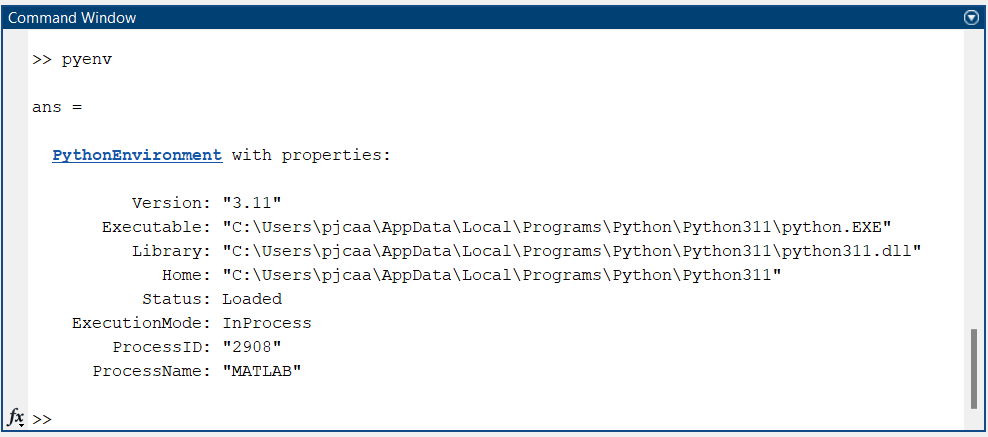
\includegraphics[width=0.85\textwidth]{Matlab_python}
	\caption{Terminal de comandos de Matlab con ejecución del comando pyversion.}
	\label{fig:Matlab_python}
\end{figure} 

\newpage
\subsubsection{Ejecución de algoritmos de Python desde Matlab}
Una vez comprobado que el entorno de trabajo de Matlab había cargado correctamente la versión de Python deseada, se procedió a verificar la capacidad de importar módulos de Python directamente en Matlab. Para ello, se realizó nuevamente un experimento de conexión y desconexión del Crazyflie. 

\vspace{5mm}
\begin{lstlisting}[caption=Algoritmo de prueba de conexión con Crazyflie., label=code:matlab_prueba1]
	import time
	import logging
	import cflib.crtp
	from cflib.crazyflie import Crazyflie
	
	def connect_crazyflie():
		cflib.crtp.init_drivers()
		logging.basicConfig(level=logging.CRITICAL)
		cf = Crazyflie(rw_cache='./cache')
		
		try:
			cf.open_link('radio://0/80/2M/E7E7E7E7E7')
			print(f"Crazyflie conectado.")
			time.sleep(5)  # Espera 5 segundos
			
		except Exception as e:
			print(f"Ocurrió un error al intentar conectar o durante la operación: {e}")
		
		finally:
			cf.close_link()
			print(f"Crazyflie desconectado.")

\end{lstlisting}

El código \ref{code:matlab_prueba1} corresponde a un script en Python con una función que realiza la conexión y desconexión del Crazyflie. Para realizar la llamada del script de Pyhton desde Matlab y ejecutar la función se utilizaron los siguientes comandos propios de Matlab:

\begin{verbatim}
	% Importa el archivo Python
	modulo = py.importlib.import_module('crazyflie_library_test');
	
	% Llama a la función desde MATLAB
	modulo.connect_crazyflie();
\end{verbatim}

El resultado obtenido se muestra en la Figura \ref{fig:Matlab_python2}, en donde se observa que en la consola de Matlab se mostraron los mensajes programados en el algoritmo de Python y se creó un objeto llamado módulo que internamente poseía las instancias de las librerías y objetos creados en el algortimo de Python. Lo que demostró que fue efectiva la ejecución e importación de algoritmos de Python directamente desde Matlab.

\vspace{5mm}
\begin{figure}[htbp]
	\centering
	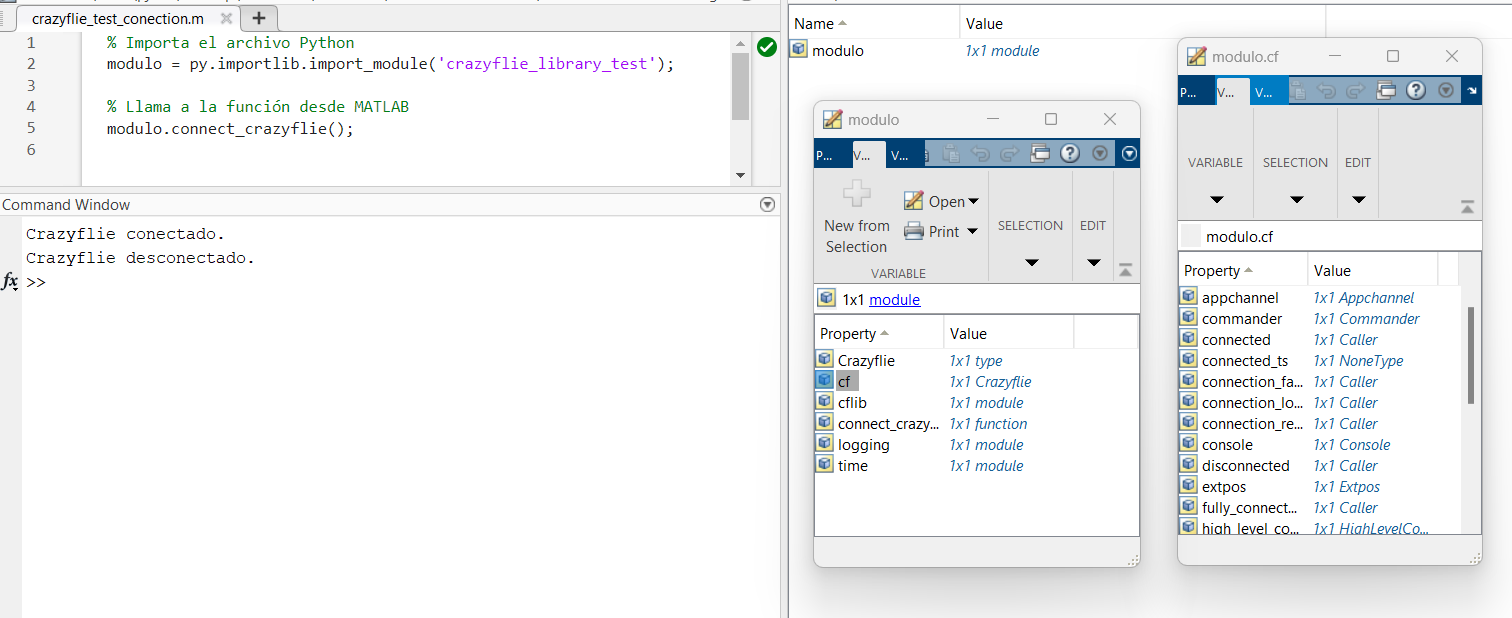
\includegraphics[width=0.9\textwidth]{Matlab_python2}
	\caption{Ejecución de script en Python de código \ref{code:prueba_conexion_crazyflie} desde Matlab.}
	\label{fig:Matlab_python2}
\end{figure} 

\subsection{Algoritmos de control en Python desde Matlab}
Una vez demostrada la correcta ejecución de algoritmos de Python desde Matlab, se desarrolló un conjunto de comandos en Matlab que permiten ejecutar funciones escritas en Python de forma directa y sencilla. Estos comandos actúan como funciones de Matlab que, internamente, llaman de manera individual a los módulos y funciones correspondientes en Python. De esta manera, es posible enviar comandos al Crazyflie sin la necesidad de interactuar directamente con Python, facilitando el uso de algoritmos de control y la realización de experimentos de vuelo complejos en el entorno conocido de Matlab.

\subsubsection{Comandos de conexión en Matlab}
\begin{itemize}
	\item crazyflie\_connect(uri)
	\item crazyflie\_disconnect(SyncCrazyflie)
\end{itemize}

\subsubsection{Comandos de lectura de variables en Matlab}
\begin{itemize}
	\item crazyflie\_get\_pose(SyncCrazyflie)
	\item crazyflie\_get\_pid\_values(SyncCrazyflie)
	\item crazyflie\_get\_pid\_x(SyncCrazyflie)
	\item crazyflie\_get\_pid\_y(SyncCrazyflie)
	\item crazyflie\_get\_pid\_z(SyncCrazyflie)
	\item crazyflie\_detect\_flow\_deck(SyncCrazyflie)
\end{itemize}

\subsubsection{Comandos de configuración de parámetros en Matlab}
\begin{itemize}
	\item crazyflie\_set\_position(SyncCrazyflie, x, y, z)
	\item crazyflie\_set\_pid\_values(SyncCrazyflie, p\_gains, i\_gains, d\_gains)
	\item crazyflie\_set\_pid\_x(SyncCrazyflie, P, I, D)
	\item crazyflie\_set\_pid\_y(SyncCrazyflie, P, I, D)
	\item crazyflie\_set\_pid\_z(SyncCrazyflie, P, I, D)
\end{itemize}

\subsubsection{Comandos de movimiento en Matlab}
\begin{itemize}
	\item crazyflie\_takeoff(SyncCrazyflie, height, duration)
	\item crazyflie\_land(SyncCrazyflie, height, duration)
	\item crazyflie\_move\_to\_position(SyncCrazyflie, x, y, z, velocity)
\end{itemize}
\vspace{5mm}
	
\subsection{Experimentos con algoritmos de control desde Matlab}
El desarrollo de los comandos de control en Matlab fue un proceso iterativo, ya que para cada comando desarrollado fue necesario realizar una serie de pruebas distintas para validar su funcionamiento bajo distintas condiciones. Una vez concluidos los comandos y verficado el funcionamiento individual, es posible realizar experimentos más complejos utilizando todos los comandos en conjunto. A continuación, se presentan algunos de los experimentos realizados:

\subsubsection{Experimento de despegue simple}
Este experimento consistió en un despegue básico, evaluando la estabilidad del dron durante la elevación y comprobando la capacidad de mantenerse en vuelo estacionario.
\vspace{5mm}
\begin{lstlisting}[caption=Algoritmo de experimento de despegue simple con Crazyflie en Matlab., label=code:prueba1_matlab]
	dron_id = 8; 
	crazyflie_1 = crazyflie_connect(dron_id);
	crazyflie_takeoff(crazyflie_1, 0.5, 2.5);
	crazyflie_land(crazyflie_1);
	crazyflie_disconnect(crazyflie_1);
\end{lstlisting}

\begin{figure}[htbp]
	\centering
	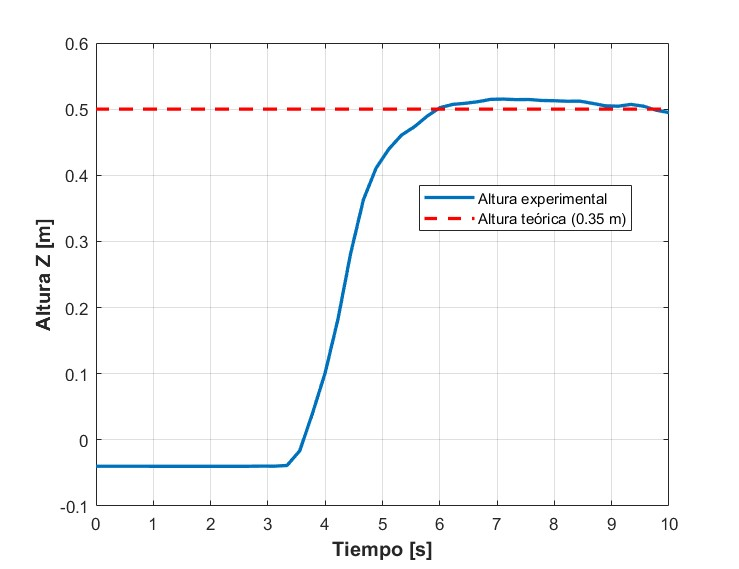
\includegraphics[width=0.65\textwidth]{takeoff}
	\caption{Gráfica de altura contra tiempo del experimento de despegue simple.}
	\label{fig:takeoff}
\end{figure} 

En la Figura \ref{fig:takeoff}, se muestra el comportamiento de vuelo para el experimento de despegue simple y evidencia el comportamiento esperado. Inicia en una altura aproximada de 0 metros y comienza a elevarse de manera progresiva hasta alcanzar la altura indicada de 0.5 metros. Este experimento se desarrolló con los valores normales para el controlador PID, por lo que vemos un comportamiento bastante estable y con error mínimo. 

\subsubsection{Experimento de despegue con modificación en el control PID de posición z}
Se realizó una modificación de los parámetros PID para el control en el eje Z durante el despegue, evaluando el impacto en la precisión y estabilidad del vuelo.
\vspace{5mm}
\begin{lstlisting}[caption=Algoritmo de experimento de despegue con modificación en el control PID de altura con Crazyflie en Matlab., label=code:prueba2_matlab]
	dron_id = 8;    
	crazyflie_1 = crazyflie_connect(dron_id);
	crazyflie_set_pid_z(crazyflie_1, 2.5, 1.5, 0.01);
	crazyflie_takeoff(crazyflie_1, 0.5, 2.5);
	crazyflie_land(crazyflie_1);
	crazyflie_disconnect(crazyflie_1);
\end{lstlisting}

\begin{figure}[htbp]
	\centering
	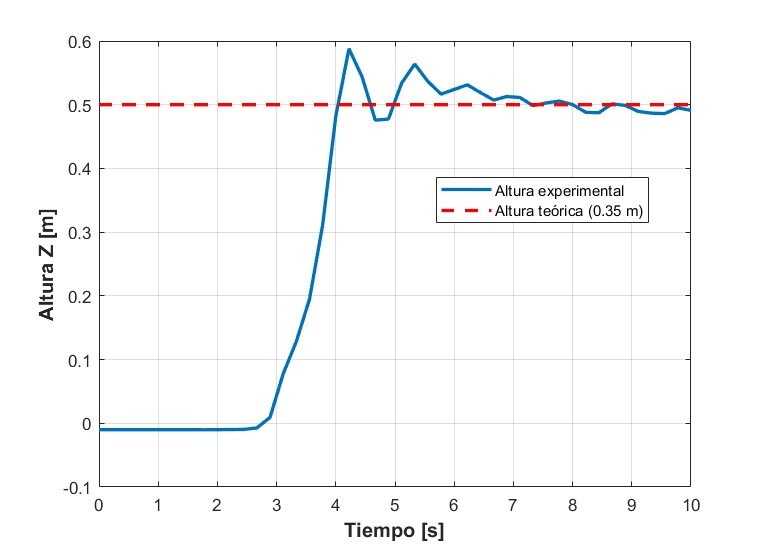
\includegraphics[width=0.65\textwidth]{takeoff_pid}
	\caption{Gráfica de altura contra tiempo del experimento de despegue con modificación de control PID de altura.}
	\label{fig:takeoff_pid}
\end{figure} 

En la gráfica de la Figura \ref{fig:takeoff_pid}, se muestra el despegue del dron Crazyflie con la modificación del control PID de altura. Tal como era esperado, se observa una variación en el comportamiento de vuelo del dron que, para el caso de los parámetros seleccionados, el comportamiento es un poco inestable. Esto se evidencia al ver que el vuelo presenta sobreimpulso al alcanzar la altura deseada, es decir, sobrepasa la altura y luego intenta estabilizarse. De esta forma, se validan las funciones de configuración de parámetros de los controladores PID de posición.

\subsubsection{Experimento de seguimiento de trayectoria circular}
En este experimento, se programó al Crazyflie para seguir una trayectoria circular.

\vspace{5mm}
\begin{lstlisting}[caption=Algoritmo de experimento de seguimiento de trayectoria circular con Crazyflie en Matlab., label=code:prueba4_matlab]
	circle_center = [0,0,0.5];
	N = 20;
	radio = 0.3;
	theta = linspace(0, 2*pi, N);  
	x = circle_center(1) + radio * cos(theta);
	y = circle_center(2) + radio * sin(theta);
	z = circle_center(3) * ones(1, N);
	
	dron_id = 8;    
	crazyflie_1 = crazyflie_connect(dron_id);
	crazyflie_takeoff(crazyflie_1, 0.3, 2.5); 
	for i = 1:N
		crazyflie_move_to_position(crazyflie_1, x(i), y(i), z(i), 0.2);
	end
	crazyflie_land(crazyflie_1);
	crazyflie_disconnect(crazyflie_1);
\end{lstlisting}

\begin{figure}[htbp]
	\centering
	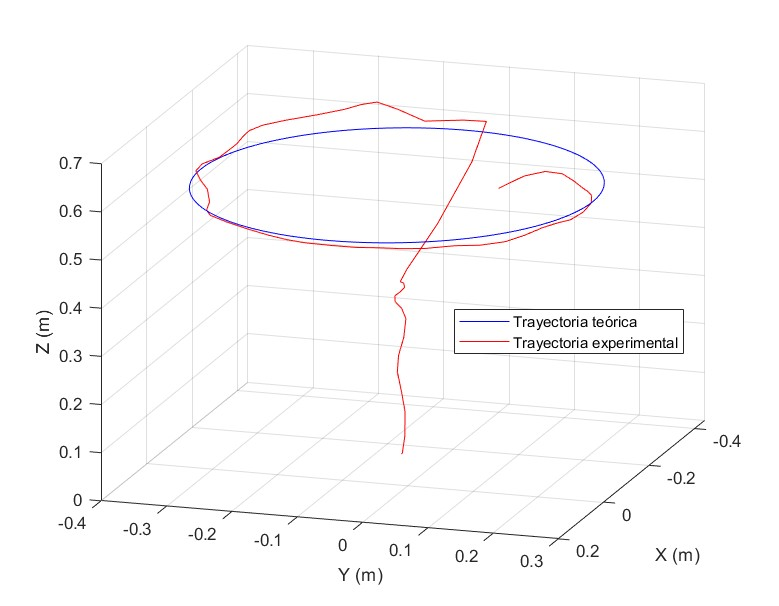
\includegraphics[width=0.65\textwidth]{Trayectoria1_FlowDeck}
	\caption{Gráfica 3D del seguimiento de trayectoria circular.}
	\label{fig:Trayectoria1_FlowDeck}
\end{figure} 

\newpage
\begin{figure}[htbp]
	\centering
	\begin{subfigure}[b]{0.4\textwidth}
		\centering
		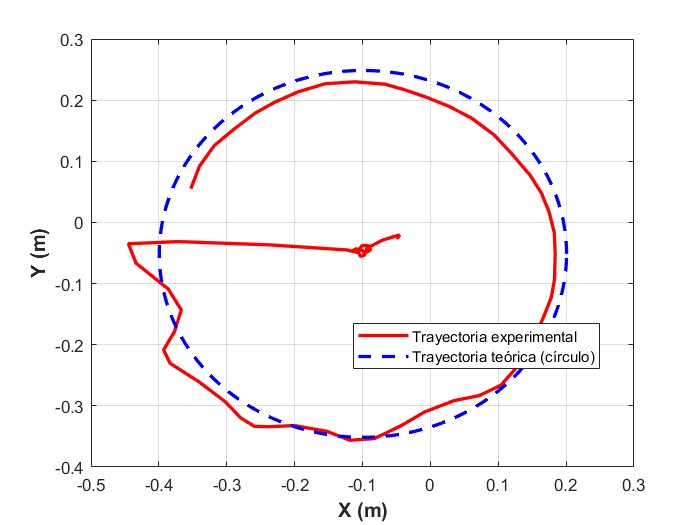
\includegraphics[width=\textwidth]{Trayectoria1_FlowDeck_xy}
	\end{subfigure}
	\hspace{0.01\textwidth} % Ajusta el espacio entre las imágenes
	\begin{subfigure}[b]{0.47\textwidth}
		\centering
		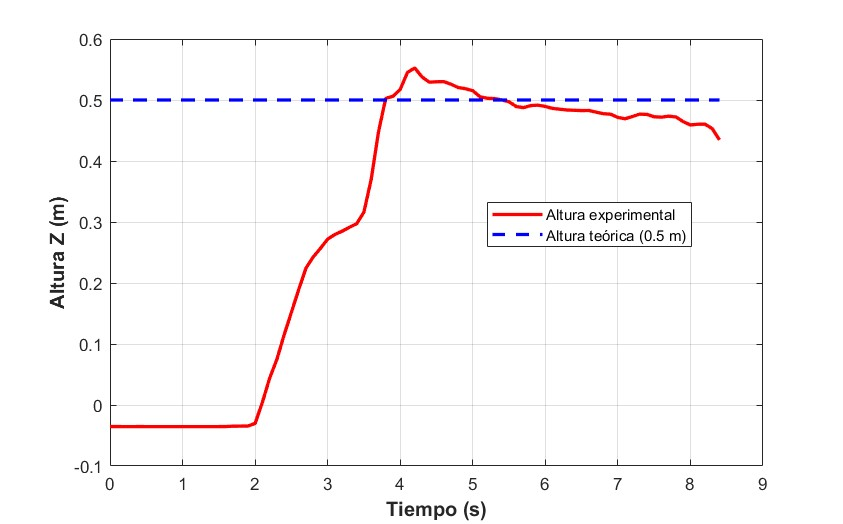
\includegraphics[width=\textwidth]{Trayectoria1_FlowDeck_z}
	\end{subfigure}
	\caption{Gráfica de posición X contra Y y gráfiza de altura contra tiempo para el seguimiento de trayectoria circular.}
	\label{fig:Trayectoria1_FlowDeck_xyz}
\end{figure}

Al analizar las gráficas mostradas en las Figuras \ref{fig:Trayectoria1_FlowDeck} y \ref{fig:Trayectoria1_FlowDeck_xyz}, se observa que el dron Crazyflie es capaz de realizar el seguimiento de las trayectorias generadas aunque no perfectamente. En la gráfica del plano X-Y, se observa que el dron experimenta desviaciones significativas en la trayectoria circular y en la gráfica de altura conta tiempo, se ve que el dron presenta una disminución progresiva de altura conforme pasa el tiempo. 

Las posibles fuentes de error incluyen limitaciones con el sensor Flow Deck, que puede verse afectado por la superficie de experimentación o la iluminación del entorno de pruebas. Aunque se intentó adaptar las condiciones del entorno para que fueran óptimas para su funcionamiento, parece que este aún presenta dificultades para posicionarse con precisión, lo que resulta en dificultades para mantener un seguimiento perfecto de la trayectoria generada. 

\newpage
\section{Fusión de sensores}
Derivado de los resultados obtenidos, se identificó que el comportamiento de vuelo podía ser mejorado de forma considerable al realizar una fusión de sensores con un sistema de posicionamiento absoluto. A raíz de ello, se intentó fusionar las lecturas de posicionamiento de la placa de expansión Flow Deck con los datos obtenidos a través del sistema de captura de movimiento del ecosistema Robotat.

Esto permitiría optimizar significativamente el rendimiento del dron, ya que las lecturas de posición relativa proporcionadas por la palca Flow Deck se complementarían con las lecturas absolutas del sistema MoCap, brindando al dron una referencia precisa de su posición dentro del entorno. Los datos de ambas fuentes serían procesados mediante el filtro extendido de Kalman para una estimación más exacta de su posición, mejorando considerablemente la precisión de vuelo del dron Crazyflie en el seguimiento de trayectorias.

\subsection{Sistema de captura de movimiento y funcionamiento desde Matlab}
El MoCap está compuesto por una red de cámaras que rastrean marcadores reflectivos adheridos a los objetos que se desean monitorear dentro del espacio controlado. Dichos marcadores permiten que el sistema calcule la posición y orientación exacta de los objetos en tiempo real respecto a una referencia absoluta. 

En el ecosistema Robotat, se utiliza una red TCP para la comunicación con el Mocap. Matlab es el software mayormente utilizado como panel de control en los laboratorios y experimentos de la universidad. Por lo tanto, es por medio de Matlab que se establece una conexión con el sistema MoCap para solicitar las poses de los marcadores reflectivos. A continuación, se listan las funciones principales para controlar el sistema:

\begin{itemize}
	\item \textbf{tcp\_obj = robotat\_connect()}: Esta función establece la conexión con la red TCP del ecosistema Robotat.
	\item \textbf{pose = robotat\_get\_pose(tcp\_obj, id\_agent)}: Solicita y devuelve la posición y orientación del marcador reflectivo especificado por id\_agent.
	\item \textbf{robotat\_disconnect(tcp\_obj)}: Finaliza la conexión con el sistema.
\end{itemize}

\subsubsection{Marcador reflectivo}
Un marcador reflectivo es un conjunto de pequeñas esferas reflectantes sujetadas sobre los cuerpos que se desean rastrear dentro del sistema. Estos marcadores están diseñados para reflejar luz emitida por las cámaras, permitiendo que el \textit{software} reconozca su posición en el espacio con alta precisión.

Para llevar a cabo la fusión de sensores de la placa Flow Deck y el sistema MoCap en el dron Crazyflie, es necesario colocar un marcador reflectivo sobre el dron. Para ello, se desarrollaron distintos prototipos de marcador que pudieran colocarse en la parte superior del Crazyflie sin afectar a las hélices y que fuera fácilmente perceptible por el sistema MoCap.

\begin{figure}[htbp]
	\centering
	\begin{subfigure}[b]{0.35\textwidth}
		\centering
		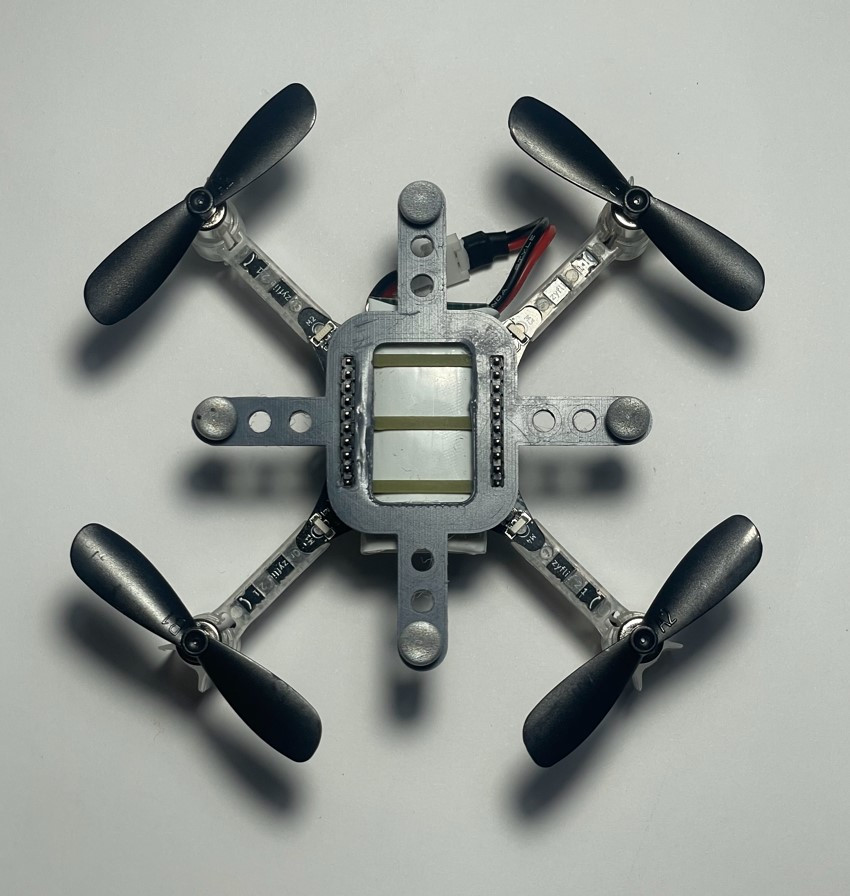
\includegraphics[width=\textwidth]{Crazyflie_marker_1}
	\end{subfigure}
	\hspace{0.01\textwidth} % Ajusta el espacio entre las imágenes
	\begin{subfigure}[b]{0.38\textwidth}
		\centering
		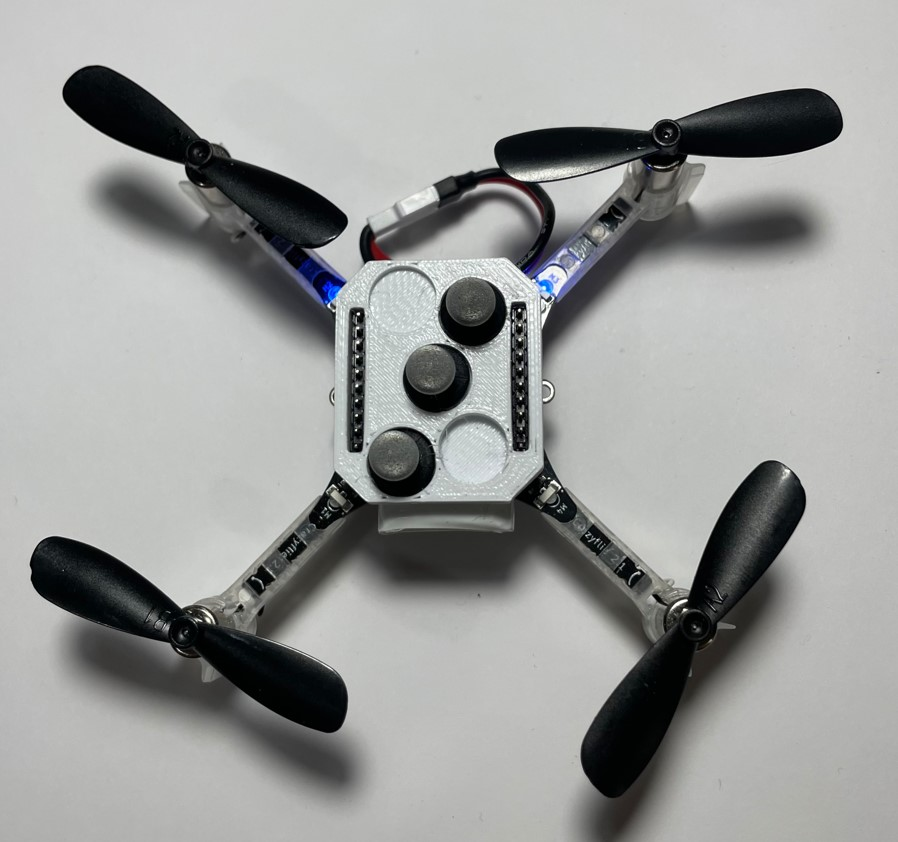
\includegraphics[width=\textwidth]{Crazyflie_marker_2}
	\end{subfigure}
	\caption{Versiones iniciales del marker para Crazyflie.}
	\label{fig:Markers_primeras_versiones}
\end{figure}

En la Figura \ref{fig:Markers_primeras_versiones} se muestran las primeras versiones desarrolladas para sujetar a las esferas reflectantes que conformarían al marcador reflectivo del dron Crazyflie. Sin embargo, presentaron cirtas dificultades al utilizar el sistema MoCap, pues en ocasiones no se registraban lecturas del cuerpo rígido. Un factor que causo esto fue que las esferas eran sobrepuestas en agujeros pero sin sostenerlas de forma definitiva, lo que ocasionaba que se movimieran milimétricamente. También, se cree que la poca distancia entre esferas dificultaba el reconocimiento del cuerpo rígido en sistema MoCap.
\vspace{5mm}
\begin{figure}[htbp]
	\centering
	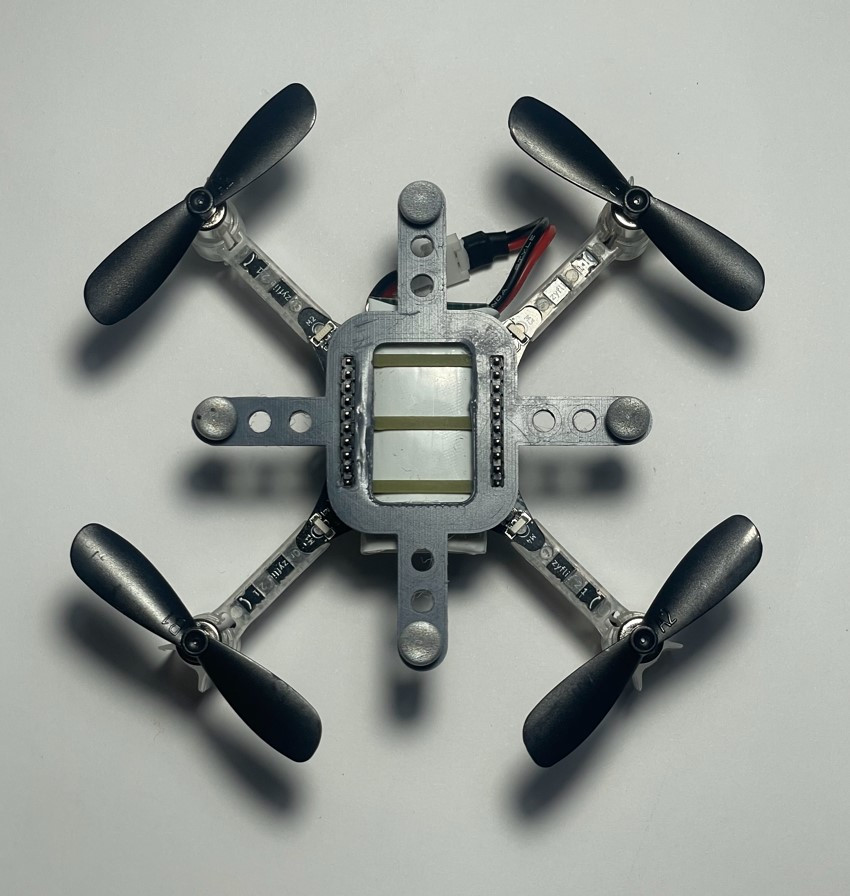
\includegraphics[width=0.4\textwidth]{Crazyflie_marker_3}
	\caption{Versión final de marcador reflectivo para dron Crazyflie.}
	\label{fig:Marker_version_final}
\end{figure} 

Tras observar estos factores, se realizó el diseño final del marcador para el dron Crazyflie, mostrado en la Figura \ref{fig:Marker_version_final}. Este dispone de agujeros para sujetar a las esferas mediante tornillos M3, de forma que la posición de estas queda totalmente rígida. Además, se utilizó una distancia considerablemente mayor entre esferas reflectivas y se añadió una esfera extra para disminuir la pérdida de reconocimiento por parte del sistema MoCap.


\subsection{Implementación de fusión de sensores}
Para la implementación de la fusión de sensores previamente descrita, se utilizó el submódulo extpos de la clase Crazyflie en la librería cflib de Python. Los datos obtenidos del sistema MoCap se enviaron mediante las funciones de este submódulo para actualizar la posición absoluta del dron, por medio del comando crazyflie\_set\_pose en Matlab. 

\subsubsection{Función de actualización de posición externa en Python}
Se desarrolló una función en Matlab que solicita las lecturas del sistema MoCap a través de la red TCP del ecosistema Robotat \ref{code:robotat_}, tal cual lo hace la función robotat\_get\_pose. Esta función también emplea del comando de actualización de posición del dron Crazyflie para completar la fusión de lecturas.

\subsubsection{Event Callback en Matlab}
Se intentó desarrollar una rutina de Event CallBack en Matlab, en la cual el evento sería la recepción de datos desde la red TCP. Sin embargo, debido a la naturaleza del sistema Robotat, que opera bajo un esquema de solicitud y recepción de información, no fue posible implementar un evento conntinuo, ya que la red TCP no envía datos de manera constante sin una solicitud previa.

\subsubsection{Sistema de corrección de posición}
Debido a la imposibilidad de implementar una fusión continua de datos en tiempo real, los datos obtenidos del sistema MoCap se utilizan de manera periódica para corregir la posición del dron. Esto compensa las desviaciones que ocurren durante el uso de la placa Flow Deck, mejorando la precisión general del dron dentro del ecosistema Robotat. 

\subsection{Pruebas de algoritmos de control con fusión de sensores desde Matlab}
Acá se describirán las pruebas ha realizarse con la mezcla de lecturas de posición...

\newpage
\begin{lstlisting}[caption=Función para actualización de posición absoluta del Crazyflie desde Matlab., label=code:robotat_]
	function robotat_update_crazyflie_position(scf, tcp_obj, agents_ids)
		max_retries = 3; 
		for attempt = 1:max_retries
			try
				timeout_count = 0;
				timeout_in100ms = 1 / 0.1;
				read(tcp_obj); 				
				if((min(agents_ids) > 0) && (max(agents_ids) <= 100))
					s.dst = 1; 
					s.cmd = 1; 
					s.pld = round(agents_ids);
					write(tcp_obj, uint8(jsonencode(s)));  
					while((tcp_obj.BytesAvailable == 0) && (timeout_count < timeout_in100ms))
						timeout_count = timeout_count + 1;
						pause(0.1);
					end					
					if(timeout_count == timeout_in100ms)
						disp('ERROR: Could not receive data from server.');
						continue;
					else
						absolute_position = jsondecode(char(read(tcp_obj)));
						absolute_position = reshape(absolute_position, [7, numel(agents_ids)])';						
						x = absolute_position(1);
						y = absolute_position(2);
						z = absolute_position(3);						
						module_name = 'crazyflie_python_commands'; 
						py_module = py.importlib.import_module(module_name);  
						py.importlib.reload(py_module);						
						try
							py_module.set_position(scf, x, y, z);
						catch ME
							error('Error using crazyflie_python_commands>set_position: %s', ME.message);
						end 						
						break;
					end
				else
					disp('ERROR: Invalid ID(s).');
					return;
				end			
			catch ME
				disp(['ERROR: ', ME.message]);
				if attempt == max_retries
					disp('Max retries reached, exiting.');
				else
					disp('Retrying...');
				end
			end
		end
	end
\end{lstlisting}

\newpage
\section{Simuladores para dron Crazyflie 2.1}
Los simuladores son herramientas cruciales en el desarrollo y prueba de algoritmos que involucran a agentes robóticos, ya que permiten simular entornos reales sin poner en riesgo el \textit{hardware} o a los experimentadores. Para el dron Crazyflie 2.1, existen algunos simuladores que permiten modelar su comportamiento en distintos escenarios, brindando un entorno seguro y flexible para experimentar con algoritmos de control y planificación de trayectorias. A continuación, se describen algunos de los simuladores utilizados que cuentan con modelos del dron Crazyflie 2.1.

\subsection{Webots}
Webots es un simulador de robots de código abierto que permite simular una amplia variedad de agentes robóticos en entornos tridimensionales. Desarrollado por Cyberbotics, Webots está diseñado para ser flexible y permite la programación de robots utilizando lenguajes como Python, C++, Java y Matlab. Es ampliamente utilizado en entornos académicos y de investigación por su capacidad de simular entornos complejos-

\subsubsection{Modelo de dron Crazyflie}
En Webots, existe un modelo del dron Crazyflie 2.1 que simula su comportamiento dinámico. Este modelo incluye herramientas para controlar al dron mediante scripts de control, lo que permite a los usuarios programar su movimiento, maniobras y experimentos con facilidad. Además, ofrece la posibilidad de integrar sensores virtuales como cámaras, IMUs y sensores de distancias.

\begin{figure}[htbp]
	\centering
	\includegraphics[width=0.85\textwidth]{Webots1}
	\caption{Simulación de modelo Crazyflie 2.1 en Webots.}
	\label{fig:Webots1}
\end{figure} 


\subsubsection{Alcance de simulaciones}


%\subsection{gym-pybullet-drones}
%Párrafo explicando qué es gym-pybullet-drones.
%\subsubsection{Modelo de dron Crazyflie}
%Párrafo explicando el modelo y herramientas disponibles para el dron Crazyflie en el simulador.
%\subsubsection{Alcance de simulaciones}

%\subsection{Nvidia Isaac}
%Párrafo explicando qué es Nvidia Isaac.
%\subsubsection{Modelo de dron Crazyflie}
%Párrafo explicando el modelo y herramientas disponibles para el dron Crazyflie en el simulador.
%\subsubsection{Alcance de simulaciones}
% ------------------------------------------------------------------------------
% CAPÍTULO 9 -------------------------------------------------------------------
% ------------------------------------------------------------------------------
\chapter{Manual de usuario y guías de laboratorio desarrolladas}
En este capítulo se presenta finalmente la elaboración de un manual de usuario e instalación de herramientas para el uso del Crazyflie 2.1 con la placa Flow Deck integrada. Asimismo, se presentan los experimentos y el desarrollo de las guías de laboratorio diseñados para los cursos de Sistemas de Control 1 y Robótica 1.

\section{Manual de usuario de Crazyflie con la placa Flow Deck}
Para cualquier equipo de laboratorio es fundamental contar con una documentación adecuada y un manual de uso que se revise previamente. Esto asegura que los usuarios comprendan cómo operar el equipo de manera segura y eficiente. En el caso del dron Crazyflie 2.1 y su placa de expansión Flow Deck, resulta indispensable disponer de un manual detallado que documente la información clave para su uso correcto durante las prácticas de laboratorio.

\subsection{Descripción}
Este manual está diseñado para guiar al usuario en el uso del dron Crazyflie 2.1 con la placa de expansión Flow Deck integrada. Proporciona instrucciones claras sobre cómo ensamblar, configurar, y operar el dron, así como las recomendaciones para el manejo de sus componentes. Además, incluye pasos detallados para la instalación de las herramientas de \textit{software} necesarias y cómo realizar pruebas básicas para verificar su funcionamiento.

\subsection{Objetivos}
\begin{itemize}
	\item Familiarizarse con el funcionamiento básico del dron Crazyflie 2.1 y la placa Flow Deck.
	\item Validar el ensamble y la instalación de la placa Flow Deck.
	\item Aprender a conectar el dron a su ordenador mediante el dispósitivo Crazyradio.
	\item Configurar las dependencias y librerías de \textit{software} necesarias para programar y controlar el dron desde Python.
	\item Realizar pruebas de conexión y verificación del funcionamiento de la placa Flow Deck, asegurando que el dron esté listo para su uso en experimentos de laboratorio.
\end{itemize}

\subsection{Prueba piloto}
\subsubsection{Descripción y condiciones de la prueba}
Acá se describirá una descripción y las condiciones en las que se desarrollará la prueba piloto.

\subsubsection{Material y Equipo Necesario}
A continuación, se presenta el listado de materiales y equipo necesarios para seguir los pasos de este manual:

\begin{itemize}
	\item Dron Crazyflie 2.1 ensamblado.
	\item Placa de expansión Flow Deck.
	\item Dispositivo Crazyradio.
	\item Ordenador con Windows 10/11.
\end{itemize}

\subsubsection{Resulados y recomendaciones}
Acá se detallarán los resultados de la prueba junto con las recomendaciones dadas. 

\newpage
\section{Guía de laboratorio para Sistemas de Control 1: Control de altura del dron Crazyflie 2.1}
\subsection{Descripción}
Este laboratorio utiliza el dron Crazyflie 2.1 como planta de estudio para implementar y ajustar controladores PID que permitan controlar su altura de vuelo. En primer lugar, los estudiantes realizarán simulaciones en MATLAB para modelar el comportamiento del dron bajo diferentes condiciones. Luego, realizarán experimentos con el dron físico, ajustando los parámetros del controlador PID y utilizando el sistema de captura de movimiento del laboratorio CIT-116 para medir y analizar su desempeño real.

\subsection{Objetivos}
\begin{itemize}
	\item Estudiar el funcionamiento del controlador PID aplicado al dron Crazyflie 2.1, analizando cómo los parámetros afectan la estabilidad y precisión del control de altura.
	\item Implementar y ajustar controladores PID en MATLAB para simular y experimentar con el control de altura del dron.
	\item Comparar los resultados obtenidos en simulaciones con los resultados obtenidos mediante la experimentación en el dron físico.
	\item Familiarizarse con el sistema de captura de movimiento del ecosistema Robotat para registrar los movimientos del dron y evaluar su rendimiento.
\end{itemize}

\subsection{Prueba piloto}
\subsubsection{Descripción y condiciones de la prueba}
Acá se describirá una descripción y las condiciones en las que se desarrollará la prueba piloto.

\subsubsection{Material y Equipo Necesario}
A continuación, se presenta el listado de materiales y equipo necesarios para seguir los pasos de este manual:

\begin{itemize}
	\item Dron Crazyflie 2.1 con la placa de expansión Flow Deck integrada.
	\item Dispositivo Crazyradio.
	\item Ordenador con Windows 10/11 con Matlab y Pyhton instalados.
	\item Paquete de herramientas de software descargado.
	\item Sistema de Captura de Movimiento del ecosistema Robotat del laboratorio CIT-116.
\end{itemize}

\subsubsection{Resulados y recomendaciones}
Acá se detallarán los resultados de la prueba junto con las recomendaciones dadas. 

\newpage
\section{Guía de laboratorio para Robótica 1: Generación y seguimiento de trayectorias con Crazyflie 2.1}
\subsection{Descripción}
En esta práctica usted aprenderá a utilizar a los drones Crazyflie 2.1 con una placa de posicionamiento relativo (Flow Deck). También, hará uso nuevamente del sistema de captura de movimiento óptico. Luego, empleará rutinas básicas en MATLAB para obtener la pose absoluta del cuerpo rígido Crazyflie para otorgarle sentido de posición absoluta al dron y finalmente realizar un experimento de seguimiento de trayectoria a través de una ruta de obstáculos.

\subsection{Objetivos}
\begin{itemize}
	\item Familiarizarse con los agentes robóticos móviles Crazyflie 2.1.
	\item Comprender a la diferencia entre un sistema de posicionamiento relativo y un sistema de posicionamiento absoluto.
	\item Familiarizarse con el sistema de captura de movimiento del ecosistema Robotat para registrar los movimientos del dron y evaluar su rendimiento.
	\item Generar trayectorias y ejecutarlas con los drones Crazyflie 2.1.
\end{itemize}

\subsection{Prueba piloto}
\subsubsection{Descripción y condiciones de la prueba}
Acá se describirá una descripción y las condiciones en las que se desarrollará la prueba piloto.

\subsubsection{Material y Equipo Necesario}
A continuación, se presenta el listado de materiales y equipo necesarios para seguir los pasos de este manual:

\begin{itemize}
	\item Dron Crazyflie 2.1 con la placa de expansión Flow Deck integrada.
	\item Dispositivo Crazyradio.
	\item Ordenador con Windows 10/11 con Matlab y Pyhton instalados.
	\item Paquete de herramientas de software descargado.
	\item Sistema de Captura de Movimiento del ecosistema Robotat del laboratorio CIT-116.
\end{itemize}

\subsubsection{Resulados y recomendaciones}
Acá se detallarán los resultados de la prueba junto con las recomendaciones dadas. 
